\documentclass[hidelinks,a4paper,12pt, nofootinbib]{article}
\usepackage[left=3cm, top=2.5cm, right=2cm, left=2.5cm]{geometry}
\usepackage[spanish, es-tabla]{babel} %es-tabla es para que ponga Tabla en vez de Cuadro en el caption
\usepackage[utf8]{inputenc}
\usepackage[T1]{fontenc}
\usepackage{xspace}
\usepackage{xargs}
\usepackage{fancyhdr}
\usepackage{lastpage}
\usepackage{caratula}
\usepackage[bottom]{footmisc}
\usepackage{amsmath}
\usepackage{amssymb}
\usepackage{algorithm}
\usepackage[noend]{algpseudocode}
\usepackage{array}
\usepackage{xcolor,colortbl}
\usepackage{amsthm}
\usepackage{listings}
\usepackage{soul}

\usepackage{pgf}

\usepackage{graphicx}
\usepackage{sidecap}
\usepackage{amsmath}
\usepackage{wrapfig}
\usepackage{caption}

%Grafos
\usepackage{tkz-berge} %Como Tikz pero más orientado a graph theory 
\usetikzlibrary{3d,arrows,automata}
\newcommand\pgfmathsinandcos[3]{% 
  \pgfmathsetmacro#1{sin(#3)}% 
  \pgfmathsetmacro#2{cos(#3)}% 
}


%Formato de los links
\usepackage{hyperref}
\hypersetup{
  colorlinks   = true, %Colours links instead of ugly boxes
  urlcolor     = blue, %Colour for external hyperlinks
  linkcolor    = blue, %Colour of internal links
  citecolor   = red %Colour of citations
}

\usepackage{comment}

%Bibliografia
\usepackage[
  backend=bibtex,
  style=alphabetic
]{biblatex}
\addbibresource{bibliografia.bib}


\captionsetup[table]{labelsep=space}


\setlength{\parindent}{4em}
\setlength{\parskip}{0.5em}


%%fancyhdr
\pagestyle{fancy}
\thispagestyle{fancy}
\addtolength{\headheight}{1pt}
\lhead{Algoritmos y Estructuras de Datos III: TP3}
\rhead{$1º$ cuatrimestre de 2016}
\cfoot{\thepage\ / \pageref{LastPage}}
\renewcommand{\footrulewidth}{0.4pt}
\renewcommand{\labelitemi}{$\bullet$}
\setcounter{section}{-1}

%%caratula
\materia{Algoritmos y Estructuras de Datos III}
\titulo{Trabajo Práctico Número 3}
%\subtitulo{}
\grupo{Grupo 8}
\integrante{Ciruelos Rodríguez, Gonzalo}{063/14}{gonzalo.ciruelos@gmail.com}
\integrante{Costa, Manuel José Joaquín}{035/14}{manucos94@gmail.com}
\integrante{Gatti, Mathias Nicolás}{477/14}{mathigatti@gmail.com}
\integrante{Maddonni, Axel Ezequiel}{200/14}{axel.maddonni@gmail.com}

\fecha{16 de Mayo de 2016}

\usepackage{etoolbox}
\AtBeginEnvironment{tikzpicture}{\shorthandoff{>}\shorthandoff{<}}{}{}

\begin{document}
\maketitle

\tableofcontents
\newpage

\section{Introducción}

En este trabajo desarrollaremos varias soluciones para el problema de el subgrafo común máximo entre dos grafos $G_1$ y $G_2$, con respecto a los vértices. 

Más precisamente, dados $G_1 = (V_1 , E_1)$ y $G_2 = (V_2 , E_2)$ dos grafos simples, el problema de máximo subgrafo común consiste en encontrar un grafo $H = (V_H , E_H)$ isomorfo tanto a un subgrafo de $G_1$ como a un subgrafo de $G_2$ que maximice $|E_H|$.

Nuestros acercamientos al problema van a ser dos. Primero, vamos a desarrollar una solución exacta, es decir, una solución que encuentra el subgrafo común que maximiza la cantidad de aristas.
Sin embargo, como veremos, esta forma de resolverlo no es razonable dado que se desconoce una solución en tiempo polinomial, por lo que encontrar la mejor solución no es viable para entradas grandes.

Luego, veremos varios algoritmos aproximados para el problema del subgrafo común máximo. Estos consisten en sacrificar exactitud a cambio de tiempo de ejecución. Su complejidad será polinomial, pero como dijimos, las soluciones que generen serán \emph{aproximadas}, o sea, no exactas.


\subsection{Experimentación}

La experimentación en general sigue los pasos sugeridos por las consignas del trabajo. Los métodos de generación de casos estarán explicados al final de cada sección de experimentación, o en su defecto, en el apéndice.

Sobre la experimentación de tiempos, como las complejidades en general dependen de muchos parámetros, los resultados se vuelven difíciles de representar.
Es por eso que seguiremos el mismo método de representación que utilizamos en los TPs anteriores.
Supongamos que la complejidad del algoritmo es $O(f(n,m))$, entonces nuestro gráfico tendrá $f(n, m)$ en el eje $x$ y $T(n, m) = \text{``El tiempo que tarda el algoritmo para una entrada de tamaño (n,m)''}$ en el eje $y$, de esta manera, nos interesará ver que el gráfico es el de una constante.

Por supuesto, también haremos experimentos en los que fijamos parámetros y movemos otros, para corroborar que las performances se comportan como deben. En caso de que las complejidades dependan de un parámetro, haremos un gráfico clásico, en caso contrario, haremos lo mismo que explicamos anteriormente.




\newpage

\section{Ejercicio 1}
\subsection{Diferencia entre MCIS y MCES}

En el paper de Ehrlich and M. Rarey se introducen técnicas de comparación de grafos moleculares, haciendo referencia al problema del MCS (maximal common subgraph). Sin embargo, el paper se enfoca en un problema diferente al planteado en este trabajo.

El problema al que hace referencia el paper es el MCIS (\textit{Maximal common induced subgraph}), es decir, dados G1 = (V1 , E1) y G2 = (V2 , E2) encontrar un grafo maximal, isomorfo tanto a un subgrafo \textbf{inducido} de G1 como a un subgrafo \textbf{inducido} de G2. Mientras que el problema planteado en este trabajo es el MCES (\textit{Maximal common edge subgraph}), es decir, un grafo isomorfo tanto a un subgrafo de G1 como a un subgrafo de G2 que maximice la cantidad de aristas.

\begin{figure}[H]
 \centering
	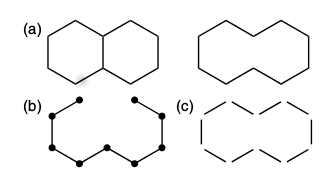
\includegraphics[width=0.7\textwidth]{img/problema1.png}
	\caption{MCIS versus MCES. Ejemplo presentado en el paper: (a) Molecular graph of
decalin (labels not shown). (b) Molecular graph of cyclodecane (labels
not shown). (c) MCIS of (a) and (b). (d) MCES of (a) and (b).}
	\label{fig:problema1-1}
\end{figure}

\subsection{Aplicaciones en la química}

Los algoritmos de MCS tienen varias aplicaciones en la ciencia molecular. En el paper se presentan varios tipos de aplicaciones: en la primera parte, se consideran algoritmos aplicados a grafos que representan moléculas orgánicas pequeñas, como drogas, mientras que en la segunda parte se mencionan aplicaciones en grafos derivados de moléculas más grandes como proteínas.

El problena del MCS es usado para medir similaridad estructural entre moléculas pequeñas, mientras que en moléculas más grandes se utilizan para calcular estructuras comunes entre moléculas. Además se menciona que a pesar de que es muy común intentar estudiar patrones comunes estructurales en moléculas de ARN (ácidos ribonucleicos), estos algoritmos no aplican demasiado.

\subsubsection{Moléculas orgánicas pequeñas}

Los algoritmos de MCS se utilizan para identificar familias de ligandos, predecir actividad de ligandos o analizar el mecanismo de reacciones. Otras aplicaciones implican alineación de ligandos, determinación de relaciones cuantitativas de propiedades estructurales y modelado farmacóforo. Algunos ejemplos son:

\begin{itemize}
\item \textbf{Clasificación de compuestos:}
Un problema central cuando se trata de pequeñas moléculas en la investigación farmacéutica es agrupar compuestos en familias o clusters según su relación estructural. Un MCS puede describir sub-estructuras comunes así como grupos funcionales entre dos moléculas. Utilizando un algoritmo para calcular el MCES se puede detectar similaridad entre compuestos que no comparten una gran sub-estructura común pero sí grupos funcionales no necesariamente conectados entre sí. A partir del número de vértices y ejes que comprende el MCS, se puede calcular un grado de similaridad entre moléculas.

\item \textbf{Predicción de actividad de compuestos:}
Una pieza clave para encontrar nuevas drogas es la identificación de compuestos químicos que muestren actividad en procesos biológicos específicos. Estudios muestran que compuestos estructuralmente similares suelen tener actividad similar, por lo que se busca identificarlos para reducir la cantidad de moléculas que deben ser testeadas experimentalmente. Las moléculas son representadas usando grafos y árboles donde los vértices representan grupos funcionales y los ejes la distribución topológica de los mismos. Se utiliza un promedio entre los valores de similaridad de los vértices comunes del MCIS entre dos compuestos para reflejar la similaridad entre las moléculas.

\item \textbf{Scaffold Hopping:}
Una desventaja de los métodos basados en similaridad para cribado virtual es su tendencia a identificar solamente compuestos que son estructuralmente similares. Sin embargo, es interesante encontrar moléculas que sean construidas desde diferentes andamios que aún preserven actividad contra el mismo tipo de proteína. Para eso se utilizan métodos de MCS sobre grafos reducidos que describen características escenciales para la actividad biológica.

\item \textbf{Mapeo de reacciones:}
Una reacción química transforma la molécula reactante al producto eliminando enlaces y formando nuevos. El método mencionado utiliza un modelado de reacciones como grafos moleculares donde los vértices son átomos y los ejes son enlaces, con pesos dados por la estabilidad de los enlaces. Usando un wMCES (weighted MCES o MCES con aristas con peso) que maximice la suma de ejes en común se puede determinar el conjunto de enlaces que fueron conservados durante la reacción con mayor probabilidad. Esto permite realizar un mapeo entre el reactivo y el producto.

\item \textbf{Determinación de relaciones cuantitativas de propiedades estructurales (QSAR):}
El concepto de QSAR es transformar conocimientos químicos en ecuaciones matemáticas que relacionen una estructura con una actividad o propiedad específica. Este modelo describe cada ligando usando valores de similaridad obtenidos por algoritmos de MCS.

\end{itemize}

\subsubsection{Proteinas}

\begin{itemize}
\item \textbf{Alineación estructural:}
La comparación estructural entre proteínas resulta muy útil para obtener información sobre la función, estabilidad y comportamiento general de las mismas. Al igual que en aplicaciones anteriores, las proteínas son modeladas con grafos y el MCES entre ellos se utiliza para describir la similaridad entre las mismas.

\item \textbf{Análisis de patrones estructurales:}
Se utiliza el MCIS para calcular la relación estructural entre dos proteínas. Esto permite investigar patrones estructurales entre proteínas relacionadas con funciones específicas.

\end{itemize}






\newpage

\section{Ejercicio 2: Algoritmo exacto}
\subsection{Explicación detallada del algoritmo}

El problema del sugrafo común máximo (con respecto a aristas) es un problema perteneciente a la clase NP, por lo que hasta el momento no se conocen algoritmos que lo resuelvan de manera exacta en tiempo polimonial. 

Por esa razón, el algoritmo que lo resuelve de manera exacta debe ser de la clase de algoritmos que exploran todo el espacio de soluciones y se quedan con la mejor. De entre esos algoritmos, elegiremos un algoritmo de backtracking, dado que proponiendo buenas podas, se pueden mejorar los tiempos de ejecución del algoritmo, evitando mirar el espacio de soluciones en su enteridad.

Nuestras soluciones, es decir, nuestos isomorfismos, van a estar representados como un vector de pares. Cada par $(v_{1i}, v_{2i})$ es un par de vértices que cumplen que $v_{1i} \in V(G_1)$ y $v_{2i} \in V(G_2)$ y nuestro isomorfismo los mapea. 

Por ejemplo, si nuestro isomorfismo es $f : V(G_1) \to V(G_2)$ tal que

$
\begin{matrix}
f(0) = f(1) \\
f(1) = f(2) \\
f(3) = f(5) \\
f(6) = f(0) \\
\end{matrix}
$

Lo vamos a almacenar de la siguiente manera: ${(0,1), (1,2), (3,5), (6,0)}$. Nótese que no importa que el ``isomorfismo'' sea parcial, dado que en realidad estamos describiendo subrafos isomorfos.

Por lo tanto, nuestro algoritmo de backtracking se va a basar en probar todas las posibles combinaciones de listas de pares, y buscar cual representa el isomorfismo con la mayor cantidad de aristas. 

Una primera poda que proponemos (bastante fácil de explicar y muy poderosa) es la que sigue: podemos notar que si ciegamente consideramos todas las combinaciones de pares, estaremos considerando todos los isomorfismos varias veces.
Por ejemplo, el vector ${(0,1), (1,2)}$ y el vector ${(1,2), (0,1)}$ representan el mismo isomorfismo, pero nuestro algoritmo naif los analizará 2 veces.

Por esta razón, diseñamos la siguiente poda: solo considerar vectores cuyo vector de primera coordenadas esté ordenado ascendentemente. En el ejemplo anterior, cuando le llegue al turno a ${(1,2), (0,1)}$, no lo analizaremos ni a él, ni a ninguno de sus descendientes, dado que todos ellos serán analizados como descendientes de ${(0,1), (1,2)}$.

Otra poda que realizamos es que, si encontramos la solución máxima posible teóricamente (es decir, la solución cuya cantidad de aristas coincide con el mínimo de las aristas de $G_1$ y $G_2$), terminar con el algoritmo inmediatamente.

Una última poda que realizamos es considerar solamente aquellos vectores cuyo largo sea exactamente el del mínimo de los vértices de $G_1$ y $G_2$. Esto se debe a que, si un vector es más chico, vamos a poder considerar a un vector extendido, cuyo isomorfismo potencialmente tendrá más aristas.

El algoritmo utiliza una variable global llamada $solucion$, que tiene 2 campos, $aristas$ e $isomorfismo$. En esta variable global irá guardando la mejor solución encontrada hasta el momendo. $solucion.aristas$ debe inicializarse en 0.

Sin más que analizar, pasemos a ver el pseudocódigo del algoritmo. Vale la pena aclarar que asumimos como preconodición que $G_1$ tiene menos nodos que $G_2$ (en tal caso de que asi no fuere, el llamador debe ocuparse de dar vuelta los parámetros).


\begin{algorithm}[H]
  \begin{algorithmic}[1]
  \caption{Pseudocódigo del procedimiento Backtracking}
  \label{algo:2-1}
    \Procedure{bt}{\texttt{Grafo} $g1$, \texttt{Grafo} $g2$, \texttt{vector<int>} $vertices1$, \texttt{vector<int>} $vertices2$, \texttt{Isomorfismo} $iso$}
      \If {$solucion.aristas == MIN(g1.m, g2.m)$}
        \Comment $O(1)$ 
        \State \Return
      \EndIf
      \If {$! ordenado\_asc(iso)$}
        \Comment $O(n_1)$ 
        \State \Return
      \EndIf
      \If {$iso.size == g1.n$}
        \Comment $O(1)$ 
        \State $aristas \gets contar\_aristas\_isomorfismo(g1, g2, iso)$
        \Comment $O(n_1^2)$ 
        \If {$aristas > solucion.aristas$}
          \Comment $O(1)$ 
          \State $solucion.isomorfismo \gets iso$
          \Comment $O(n_1)$ 
          \State $solucion.aristas \gets aristas$
          \Comment $O(1)$ 
        \EndIf
        \State \Return
      \EndIf
      
      \For {$u \in vertices1$}
        \Comment $v_1$ veces $O(1)$ 
        \For {$v \in vertices2$}
          \Comment $v_1 v_2$ veces $O(1)$ 
          \State $nuevo\_iso = iso$
          \Comment $v_1 v_2$ veces $O(n_1)$ 
          \State $nuevo\_iso.push\_back(make\_pair(u,v))$
          \Comment $v_1 v_2$ veces $O(1)$ 
          \State $bt(g1, g2, copiar\_sin(vertices1, u), copiar\_sin(vertices2, v), nuevo\_iso)$
          \Comment $v_1 v_2$ veces $T(n_1, n_2, v_1 - 1, v_2 - 1)$
        \EndFor
      \EndFor
		\EndProcedure
	\end{algorithmic}
\end{algorithm}



\begin{algorithm}[H]
  \begin{algorithmic}[1]
  \caption{Pseudocódigo del procedimiento contar aristas isomorfismo}
  \label{algo:2-2}
    \Procedure{contar\_aristas\_isomorfismo}{\texttt{Grafo} $g1$, \texttt{Grafo} $g2$, \texttt{Isomorfismo} $iso$} $\to$ \texttt{Int}
      \State $aristas \gets 0$
      \Comment $O(1)$
      \For {$ p \in iso$}
         \Comment $n_1$ veces $O(1)$ 
         \State $vg1 = p.first$
         \Comment $n_1$ veces $O(1)$ 
         \State $vg2 = p.second$
         \Comment $n_1$ veces $O(1)$ 
         \For {$q \in iso$}
           \Comment $n_1$ veces $O(1)$
           \State $ug1 = q.first$
           \Comment $n_1^2$ veces $O(1)$
           \State $ug2 = q.second$
           \Comment $n_1^2$ veces $O(1)$
           \If {$g1.adj\_matrix[vg1][ug1] \land g2.adj\_matrix[vg2][ug2]$}
           \Comment $n_1^2$ veces $O(1)$
             \State $aristas++$
             \Comment $n_1^2$ veces $O(1)$
           \EndIf
         \EndFor
       \EndFor
     \Return aristas
		\EndProcedure
	\end{algorithmic}
\end{algorithm}

Donde $n_i = |V(G_i)|$ y $m_i = |E(G_i)|$, para $i = 1, 2$. Nótese que el largo del vector isomorfismo está acotado superiormente por $n_1$, pues $n_1 < n_2$ y el isomorfismo mapea a lo sumo a todos los vértices de $n_1$ y no puede mapear más cosas. 

Además, $v_i$ para $i = 1,2$ es el tamaño del vector $verticesi$.


El algoritmo debe ser llamado de la siguiente manera:

\[bt(grafo1, \{1,...,|V(grafo1)|\}, grafo2, \{1,...,|V(grafo2)|\}, \{ \})\].

Dado que inicialmente tódos los vértices están sin ser utilizados, y el isomorfismo es el isomorfismo vacío.

\subsubsection{Complejidad del algoritmo}

Calculemos la complejidad del algoritmo. Primero, como vimos, la complejidad del algoritmo contar\_aristas\_isomorfismo es $O(n_1^2)$ y es bastante fácil de calcular.

Ahora, calculemos la complejidad del algoritmo de backtracking. Sea $T(n_1, n_2, v_1, v_2)$ el tiempo que el algoritmo tarda para una entrada de ese tamaño. El tamaño del vector $iso$ puede acotarse por $n_1$, como vimos antes.

Como se ve en en análisis de complejidad, $T(n_1, n_2, v_1, v_2) = n_1 + n_1^2 + v_1 v_2 n_1 + v_1 v_2 + v_1 v_2 T(n_1, n_2, v_1 - 1, v_2 - 1)$.

Además, notemos que siempre pasa que $v_i < n_i$, luego, la complejidad puede acotarse por $T(n_1, n_2, v_1, v_2) < n_1 + n_1^2 + v_1 v_2 n_1 + v_1 v_2 + v_1 v_2 T(n_1, n_2, v_1 - 1, v_2 - 1)$.
Nos tomamos la libertad de escribir $T(v_1, v_2)$, dado que son los únicos parámetros variables ($n_1$ y $n_2$ están fijos).


Como $n_i > v_i$, $T(v_1, v_2) < n_1 + n_1^2 + n_1 n_2 n_1 + n_1 n_2 + v_1 v_2 T(v_1 -1, v_2 - 1)$. 

Luego, $T(v_1, v_2) < 4 n_1^2 n_2 + v_1 v_2 T(v_1 -1, v_2 - 1)$.

Además, $T(n_1, n_2, 0, v_2) = n_1 + n_1^2$ (recordemos que siempre va a pasar que $n_1 < n_2$, por lo tanto $v_1 < v_2$). Por lo que la profundidad de la fórmula recursiva depende solo de $v_1$. Luego,
\[
\begin{array}{ll}
T(v_1, v_2) & < 4 n_1^2 n_2 + v_1 v_2 T(v_1 - 1, v_2 - 1) \\
  & < 4 n_1^2 n_2 + v_1 v_2 (4 n_1^2 n_2 + (v_1-1)(v_2-1) T(v_1-2,v_2-2)) \\
  & = 4 n_1^2 n_2 + v_1 v_2 4 n_1^2 n_2 + v_1 v_2 (v_1-1)(v_2-1)T(v_1-2,v_2-2) \\
  & < 4 n_1^2 n_2 + 4 n_1^3 n_2^2 + v_1 v_2 (v_1-1)(v_2-1)T(v_1-2,v_2-2) \\
  & < ... \\ 
  & < 4 n_1^2 n_2 + ... + 4 n_1^{v_1} n_2^{v_1 - 1} + v_1 (v_1 - 1) ... (v_1 - v_1 + 1)  v_2 (v_2 - 1) ... (v_2 - v_1 + 1) T(0, v_2 - v_1) \\ 
  & < 4 n_1^2 n_2 + 4 n_1^3 n_2^2 + ... + 4 n_1^{v_1} n_2^{v_1 - 1} + 4 n_1^{v_1 + 1} n_2^{v_1}  \\
  & < 4 n_1^2 n_2 + 4 n_1^3 n_2^2 + ... + 4 n_1^{v_1+1} n_2^{v_1} \\
  & < 4^{v_1 + 1} n_1^{v_1+1} n_2^{v_1 + 1} \\ 
  & = (4 n_1 n_2)^{v_1 + 1} \\
\end{array}
\]

Luego, $T(n1, n2) \in O((4 n_1 n_2)^{n_1 + 1})$.

Nótese que esta es una cota bastante poco ajustada, pero es suficientemente exacta para el análisis que queremos hacer (una cota más ajustada, como se ve en los cálculos anteriores, involucra fórmulas con factoriales y combinatorios).



\subsection{Performance del algoritmo}

Asdf


\newpage

\section{Ejercicio 3}
\subsection{Problema del MCS entre cografos y grafos completos}

En esta sección se presenta un algoritmo exacto para resolver el problema en cuestión para el caso particular en que los dos grafos de entrada son un cografo y un grafo completo, respectivamente. El problema del MCS para este tipo de grafos de entrada puede resolverse en tiempo polinomial, debido a características particulares de este tipo de grafos.

En principio, si consideramos el problema del MCS entre un grafo cualquiera G y un grafo completo Kn, se deduce fácilmente que si $|Kn| \geq |G| \Rightarrow MCS(G, Kn)$ = $G$. Por lo tanto, el caso interesante que se busca resolver es cuando $|G|$ > $|Kn|$.

Para esto, el algoritmo presentado aprovecha la siguiente definición recursiva de un cografo:

\emph{def. \textbf{Cografo}
\begin{enumerate}
\item El grafo trivial es un cografo.
\item La unión ( $\cupdot$ ) disjunta de dos cografos es un cografo.
\item El join ( $\lor$ ) de dos cografos es un cografo, donde $G1 \lor G2 = \overline{\overline{G1} \cupdot \overline{G2}}$.
\end{enumerate}
}

\subsection{Explicación detallada del algoritmo}

El algoritmo propuesto utiliza la técnica de programación dinámica. Aprovechando la definición recursiva de los cografos, dividimos el problema en subproblemas más chicos. Dada la definición, un cografo puede ser un grafo trivial, unión o join de dos cografos. 
Se define la siguiente función recursiva:

$f(G, K, i) = MCS(G, K)$ usando $i$ nodos, con $i \leq min \{|G|, |K|\}$

donde:

\[ f(G, K, i) = \begin{cases} \label{formulacionRecursiva}
      G & si\ G\ trivial \\
      \underset{0 \leq j \leq i}{maxAristas}\ \{ MCS(G1, K, j) \cupdot MCS(G2, K, i-j)\}
      & si\ G = G1 \cupdot G2 \\
      \underset{0 \leq j \leq i}{maxAristas}\ \{ MCS(G1, K, j) \lor MCS(G2, K, i-j)\}
      & si\ G = G1 \lor G2
   \end{cases}
\]

La solución que buscamos, entonces, es: $f(G, K, min \{|G|, |K|\})$.

\subsubsection{Correctitud de la formulación recursiva}

\begin{itemize}
\item \textbf{Caso trivial.} El MCS de un grafo trivial con un grafo completo es ($\{v\}$, $\{\}$), donde $v$ es el único nodo de $G$.
\item \textbf{Caso $G$ es unión de cografos $G1, G2$.} Por transitividad, MCS($Gi, K, j$) $\in G$ pues es subgrafo de $Gi$ y $Gi$ es subgrafo de $G$ $\forall i \in (1,2)$. Además, toda arista y nodo del $MCS(G,K,j)$ de $j$ vertices pertenece bien a $G1$ o a $G2$. Por lo que podemos calcularlo quedándonos con el MCS de máxima cantidad de aristas resultante entre todas las combinaciones posibles de usar $x$ cantidad de nodos de $G1$ y $j-x$ nodos de $G2$ ($x \in [0..j]$). Para ver cuál es el mejor MCS resultante es necesario calcular el x que maximice la cantidad de aristas de la unión entre los $MCS(G1,K,x)$  y $MCS(G2,K,j-x)$ (para todo $x$ válido), ya que vale el principio de optimalidad. Si utilizáramos otro subgrafo de $G1$ o $G2$ que no fuera MCS del mismo, entonces el MCS resultante para $G$ no sería óptimo, pues podríamos intercambiarlo por el óptimo y obtener un MCS mejor para $G$.
\item \textbf{Caso $G$ es join de cografos $G1, G2$.} Para este caso, debemos considerar las aristas que se agregan al hacer el join. Al igual que en el caso anterior, todo nodo del $MCS(G,K,j)$ de $j$ vertices pertenece bien a $G1$ o a $G2$. Por lo que podemos calcularlo quedándonos con el MCS de máxima cantidad de aristas resultante entre todas las combinaciones posibles de usar $x$ cantidad de nodos de $G1$ y $j-x$ nodos de $G2$ ($x \in [0..j]$). Sin embargo, no podemos quedarnos con la unión de los MCS de los subgrafos tal que la suma de las aristas es la máxima como en el caso anterior, ya que hay aristas que no estamos considerando. Éstas aristas son las aristas que se agregan cuando se realiza el join entre dos grafos, y son todas aquellas que unen cada nodo de una componente del join a todos los nodos de la otra. Por lo que, para calcular la mejor combinación posible de nodos entre $G1$ y $G2$ debemos sumar la cantidad de aristas entre el $MCS(G1,K,x)$  y $MCS(G2,K,j-x)$. Entonces, buscamos la combinación que maximice lo siguiente:
\[ aristas(MCS(G1,K,x)) + aristas(MCS(G2,K,j-x)) + x*(j-x) \forall x \in [0..j] \]
donde $x*(j-x)$ corresponde a la cantidad de aristas con un extremo en $G1$ y otro en $G2$. Al igual que en el caso anterior, si utilizáramos otro subgrafo de $G1$ o $G2$ que no fuera MCS del mismo, entonces el MCS resultante para $G$ no sería óptimo, pues podríamos intercambiarlo por el óptimo y obtener un MCS mejor para $G$.
\end{itemize}
$\qed$

Como hay soluciones que se deben calcular más de una vez, utilizando programación dinámica nos guardamos las soluciones parciales resueltas para utilizar luego, reduciendo la complejidad final del algoritmo. Para implementar esta función, se realizó una implementación de una clase \emph{CographTree} basada en una estructura de árbol binario de cografos, para representar el grafo de entrada, y poder aplicar la recursión. La raíz del árbol es el cografo original de entrada, y tiene dos cografos hijos en caso de ser unión o join de éstos (las hojas del árbol son grafos triviales). 

A grandes rasgos, el algoritmo para resolver este problema se divide en 4 partes:
\begin{enumerate}
\item Lectura de entrada
\item Generación de la estructura \emph{CographTree} a partir del grafo de entrada
\item Cálculo del MCS
\item Impresión de la solución 
\end{enumerate}

A diferencia del resto de los algoritmos, los datos de entrada se guardan en una estructura \emph{Grafo\_adjlist} basada en una lista de adyacencias. Dicha estructura utiliza un diccionario(nodo, lista<nodos> ) para representar un grafo. Esta estructura permite, una vez calculados los nodos correspondientes al MCS, calcular fácilmente el subgrafo inducido por dichos nodos en el grafo original, manteniendo la numeración original de los nodos.

\subsubsection{Generación del CographTree}

A continuación se encuentra el pseudocódigo de la función utilizada para inicializar el CographTree correspondiente al grafo de entrada:

\begin{algorithm}[H]
  \begin{algorithmic}[1]
  \caption{Pseudocódigo del constructor de CographTree}
  \label{algo:3-1}
  \Procedure{CographTree}{\texttt{Grafo\_adjlist} $g$}
	\State $n = g.n$
	\State $m = g.m$
	\State $nodos = nodosIds(g)$
	\State $sol = <false, Solucion>(n+1)$
	\State \Comment El vector sol se utiliza para almacenar las soluciones parciales usando de 0 a g.n nodos. Se inicializa en false para indicar que la dicha solución todavía no fue resuelta.
	\State $componentes = obtenerComponentesCografo(g, false)$
	\If {$|componentes| == 2$}
		\State $tipo = unionDisjunta$
		\State $izq = CographTree(subgrafoInducido(g, componentes[0])$
		\State $der = CographTree(subgrafoInducido(g, componentes[1])$
	\ElsIf {$|componentes| == 1$}
		\State $tipo = trivial$
		\State $izq = null$
		\State $der = null$
	\Else
		\State $tipo = join$
		\State $componentesJoin = obtenerComponentesCografo(g, true)$
		\State $izq = CographTree(subgrafoInducido(g, componentesJoin[0])$
		\State $der = CographTree(subgrafoInducido(g, componentesJoin[1])$
	\EndIf
	\EndProcedure
	\end{algorithmic}
\end{algorithm}

El algoritmo se basa primero en verificar si el cografo de entrada es conexo. En caso de que no lo sea, entonces por definición el cografo es unión de otros dos (un join de dos grafos siempre es conexo, ver demostración debajo). Si el cografo es conexo, puede ser un grafo trivial o un join de otros dos cografos.

\emph{\textbf{dem.}} \textit{Sea $G$ un grafo tal que $G = G1\ \lor\ G2$, $\Rightarrow$ $G$ es conexo.} Sea $v$ un vértice cualquiera. Por definición de join, $\forall v \in G1, u \in G2, \exists (u, v) \in G$. Spge, asumo $v \in G1$. Entonces, existe un camino desde $v$ a todos los nodos pertenecientes a $G2$, ya que está conectado a todos ellos. Sea $u$ un nodo $\in G2$. Por la misma razón $u$ está conectado a todos los nodos de $G1$. Por lo tanto existe un camino desde $v$ a todos los demás nodos de $G1$ pasando por $u$. Entonces, $G$ es conexo.$\qed$

Para verificar si el grafo es conexo, se calculan las componentes conexas llamando a \emph{obtenerComponentesCografo}. Esta función está basada en BFS, pero a diferencia de éste, si el grafo tiene más de dos componentes conexas: $C_1, C_2, ..., C_k$, sólo devuelve dos componentes, $C'_1 = C_1$ y $C'_2 = C_2 \cup C_3 \cup ... \cup C_k$. De esta manera se logra que el CographTree generado finalmente sea binario. El segundo parámetro de la función es un booleano que se usa para indicar si lo que se buscan son las dos componentes de un cografo Join. (es decir se buscan $G1, G2$ tal que $G = G1 \lor G2$). Para esto, se introduce una modificación al BFS, tal que en lugar de recorrer los adyacentes a cada nodo, se recorren los nodos no adyacentes de los mismos, para calcular los nodos correspondientes a uno de los grafos del join. A continuación una demostración de que el algoritmo con dicha modificación calcula efectivamente las dos componentes de un join.

\emph{\textbf{dem.}} Dado $G, G1, G2$ grafos, tal que $G = G1\ \lor\ G2$. Es decir, $\forall v \in G1, u \in G2, \exists (u, v) \in G$. Comenzando con un nodo aleatorio $x$, marco todos los nodos no adyacentes. Spge, supongo $x \in G1$. Estos nodos se encuentran necesariamente en G1, ya que $x$ es adyacente a todos los nodos de G2. Luego, marco los nodos no adyacentes a dichos nodos, que también, por la misma razón, pertenecen a G1. De esta manera, iterativamente, marcamos todos los nodos pertenecientes a G1. El resto de los nodos que quedó sin marcar, pertenece a la otra componente del join.$\qed$

Una vez determinadas las dos componentes del cografo (sea unión o join), se aplica recursivamente para construir los cografos correspondientes a los subgrafos inducidos por los nodos de dichas componentes y continuar armando el árbol de cografos hasta completar las $n$ hojas con grafos triviales.

Notar que la estructura \texttt{CographTree} sólo almacena los ids de los nodos del grafo original, y no las adyacencias. Esto basta ya que una vez calculada la solución puede obtenerse el subgrafo inducido por los nodos de la misma sin necesidad de almacenar y recalcular las adyacencias de cada cografo del árbol.

\subsubsection{Pseudocódigo del algoritmo MCS para cografos}

A continuación, el pseudocódigo de la función para calcular el MCS dado una cantidad de nodos y el tamaño del grafo completo: (notar que la función devuelve los ids de los nodos del grafo original que corresponden al MCS).

\begin{algorithm}[H]
  \begin{algorithmic}[1]
  \caption{Pseudocódigo de MCS entre Cografo y Grafo Completo}
  \label{algo:3-2}
  \Procedure{mcs\_sol}{\texttt{CographTree} $cografo$, \texttt{int} $cantNodos$, $tamGrafoCompleto$ } $\to$ \texttt{Solucion: <cantAristasSol, nodosSol>}
    	\If { $cantNodos > cografo.n$ }
  		\State return $mcs\_Sol(cografo.n, tamGrafoCompleto)$
  	\Else
  		\State \texttt{int} $cantAristasSol$
  		\State \texttt{vector<int>} $nodosSol$
  		\If { $cantNodos == 0$ }
  			\State $cantAristasSol = 0$
  		\ElsIf { $cografo.sol[cantNodos].resuelto?$ }
  			\State return $cografo.sol[cantNodos].solucion$
  		\ElsIf { $cantNodos == 1 \ OR\  cografo.tipo == trivial$ }
  			\State $cantAristasSol = 0$
  			\State $nodosSol = cografo.nodos[0]$
  		\ElsIf { $cografo.n \leq tamGrafoCompleto \ AND\ cantNodos == cografo.n$ }
  			\State $cantAristasSol = 0$
  			\State $nodosSol = cografo.nodos$
  		\Else
  			\State \texttt{int} $maxAristas = 0$
  			\For { $i \in [0 .. cantNodos]$ }
  				\State $solIzq = mcs\_Sol(cografo.izq, i, tamGrafoCompleto)$
  				\State $solDer = mcs\_Sol(cografo.der, cantNodos-i, tamGrafoCompleto)$
  				\State $aristas = solIzq.cantAristas + solDer.cantAristas$
  				\If { $cografo.tipo == join$ }
  					\State $aristas += |solIzq.nodosSol| * |solDer.nodosSol|$
  				\EndIf
  				\If { $aristas > maxAristas \ AND \ \newline ( |solIzq.nodosSol| + |solDer.nodosSol| == cantNodos)$ }
  					\State $maxAristas = aristas$ 
  					\State $nodosSolIzq = solIzq.nodosSol$
  					\State $nodosSolDer = solDer.nodosSol$
  				\EndIf
  			\EndFor
  			\State $cantAristasSol = maxAristas$
  			\If { $cantAristasSol == 0$ }
  				\For { $i \in [0..cantNodos)$ }
  					\State $nodosSol.agregar(nodos[i])$
  				\EndFor
  			\Else
  				\State $nodosSol = unirNodos(nodosSolIzq, nodosSolDer)$
  			\EndIf
  		\EndIf
  		\State \texttt{Solucion} $s = <cantAristasSol, nodosSol>$
  		\State $cografo.sol[cantNodos].resuelto? = true$
  		\State $cografo.sol[cantNodos].solucion = s$
  		\State return $s$
  	\EndIf
  \EndProcedure
  \end{algorithmic}
\end{algorithm}

\subsection{Complejidad del Algoritmo}

La complejidad del algoritmo se puede calcular como:
C (Leer entrada) + C (Generación de CographTree) + C (MCS) + C (Imprimir)

\begin{itemize}
\item \texttt{Leer entrada.} $ O (n + m) $ 
\item \texttt{Generación de CographTree.} Para generar esta estructura recursiva, es necesario inicializar cada cografo del árbol. 
Para eso, para cada uno de ellos se ejecuta \hfill \break
\texttt{obtenerComponentesCografo} al menos una vez para chequear si el grafo correspondiente es conexo usando BFS $O(n+m)$.
Además, si el grafo es conexo se ejecuta con la modificación sobre el BFS, recorriendo los nodos no adyacentes en lugar de los adyacentes. Con esta modificación, la complejidad del algoritmo es $O(n^2)$.
Por lo tanto la complejidad quedaría:
\begin{align*}
\sum_{i=1}^{tam(CographTree)} O ( (n_i)^2 + m_i ) & = \\
& = O ( tam(CographTree) * n^2 ) +  O ( tam(CographTree) * m ) \\
\intertext{ notar que la suma de los $n_i$ y los $m_i$ pertenecientes a cada nivel del CographTree es $O(n)$ y $O(m)$ respectivamente.}
& = O ( n * n^2 ) +  O ( n * m ) \\
\intertext{ acotamos $tam(CographTree)$ por $n$ pues el cotree tiene obviamente $n$ hojas (una por cada nodo) y como es binario completo, la cantidad de nodos es aproximadamente $2n$.}
& = O ( n^3 + n*m )
\end{align*}

donde $n_i$ y $m_i$ son los correspondientes al $i$-ésimo cografo del CographTree.

\item \texttt{MCS.} Por cada cografo del CographTree debemos chequear cuál es la mejor combinación de nodos, para eso debemos probar con $n_i$ posibles combinaciones. Cada solución parcial se resuelve una sola vez, ya que vamos guardando las soluciones en el vector \texttt{sol}. Por lo que la complejidad queda:
\begin{align*}
\sum_{i=1}^{tam(CographTree)} O (n_i) & = \\
& = O ( tam(CographTree) * n ) \\
& = O ( n * n ) \\
& = O ( n^2 ) \\
\end{align*}

\item \texttt{Imprimir.} $O( min( n, n_K) + min (m, m_K) )$, donde $n_K$ y $m_K$ corresponden al grafo completo de entrada.
\end{itemize}

La complejidad total queda: 
$O( n^3 + n*m + min( n, n_K) + min (m, m_K) )$

\subsection{Performance del Algoritmo}

Confirmemos experimentalmente las complejidades enunciadas anteriormente. Como siempre, dejamos de lado la parte de entrada salida, dado que hace que la varianza sea muy alta, y no vale la pena en general medir esta parte porque no es lo central del algoritmo. Por lo tanto, esperaremos que lo que medimos tenga complejidad $O(n^3 + nm)$. 

Para experimentar, utilizamos el algoritmo de generación de cografos al azar que analizaremos en la siguiente sección. Medimos los tiempos manualmente, y los graficamos como explicamos en la introducción. 

\begin{figure}[H]
 \centering
	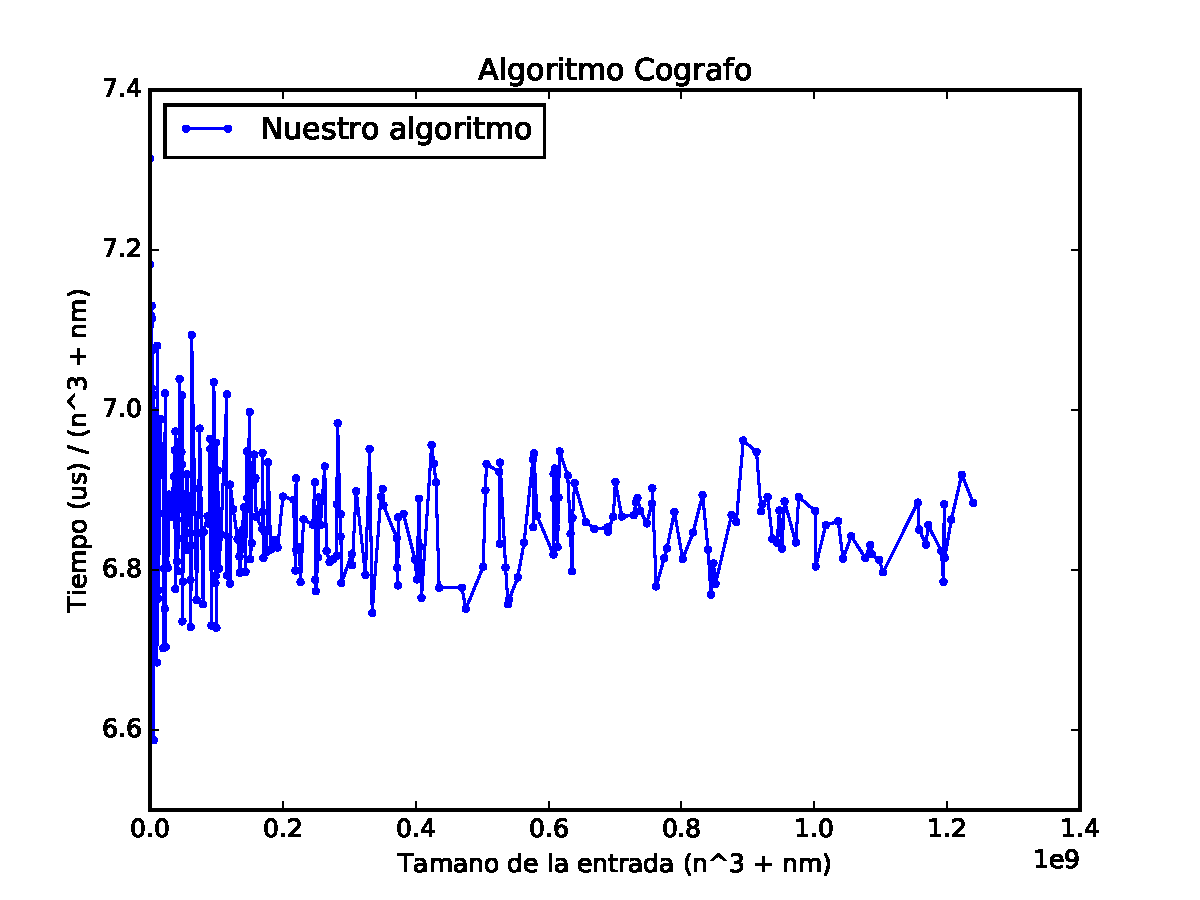
\includegraphics[width=0.8\textwidth]{graficos/problema_3/tiempos0.pdf}
	\caption{}
	\label{fig:problema3-tiempos0}
\end{figure}

Con este experimento confirmamos lo que esperabamos, dado que se ve que el cociente entre tiempo y tamaño de entrada está acotado por una constante, que es lo que queremos que pase, como dijimos en la introducción.

Además, podemos comprobar que si fijamos $n$, todo anda como debería, es decir, la complejidad es lineal en $m$.

\begin{figure}[H]
 \centering
	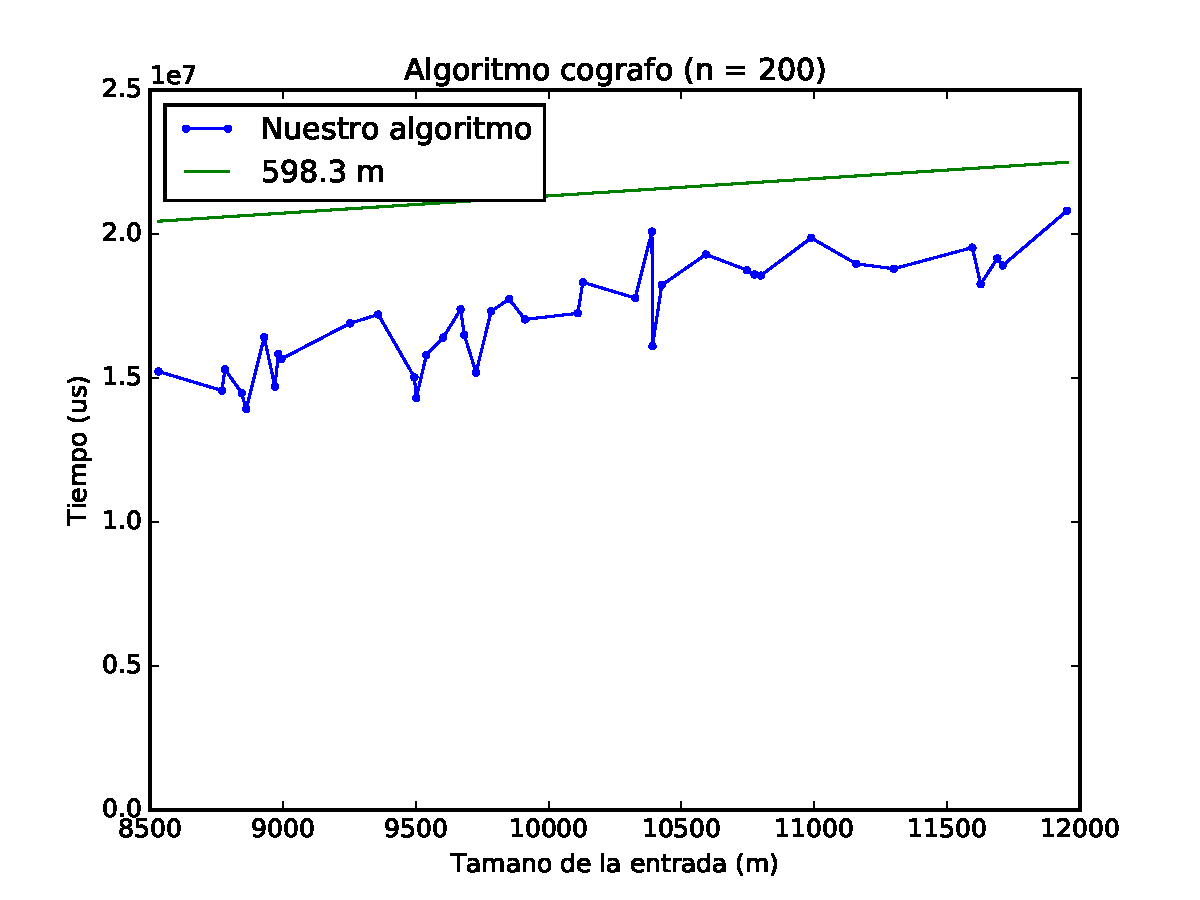
\includegraphics[width=0.8\textwidth]{graficos/problema_3/tiempos1.pdf}
	\caption{}
	\label{fig:problema3-tiempos1}
\end{figure}

Por último, por completitud, es importante decir que es muy díficil, de hecho imposible, hacer el experimento en el que se fija $m$ y se varia $n$, porque nada nos garantiza  que existan suficientes cografos con cantidad de aristas $m$ de distinto $n$ como para hacer un experimento significativo, y además no es claro como generarlos (es decir, dado un $m$ como encontrar todos o varios cografos de distintos $n$).


\subsection{Generación y testing de casos random}

Para testear la correctitud del algoritmo, primero se ejecutó el mismo con grafos de entrada más chicos y se comparó la solución con el algoritmo exacto (Problema anterior). Además, se implementó un generador de cografos random para calcular la performance, testear la correctitud y utilizar como parámetro de comparación en la posterior experimentación de las heurísticas.
A continuación se presenta un algoritmo para generar cografos de manera random:

\begin{algorithm}[H]
  \begin{algorithmic}[1]
  \caption{Pseudocódigo del constructor random de un CographTree}
  \label{algo:3-3}
  \Procedure{CographTree}{\texttt{int} $size$, \texttt{int} $nodoInicial$}
	\State \Comment $nodoInicial$ corresponde al id del primer nodo.
	\State $n = size$
	\For { $i \in [nodoInicial .. nodoInicial + size]$ }
		\State $nodos.agregar(i)$ 
	\EndFor
	\State $sol = <false, Solucion>(n+1)$
	\If { $size == 1$ }
		\State $tipo = trivial$
		\State $izq = null$
		\State $der = null$
	\Else
		\State $nodosIzq = (rand()$ \texttt{mod} $(n-1)) + 1 $
		\State $nodosDer = n - nodosIzq$
		\State $izq = CographTree(nodosIzq, nodoInicial)$
		\State $der = CographTree(nodosDer, nodoInicial + nodosIzq)$
		\State \texttt{int} $trand = rand()$ \texttt{mod} $2$
		\If { $trand == 0$ }
			\State $tipo = unionDisjunta$
			\State $m = izq.m + der.m$
		\Else
			\State $tipo = join$
			\State $m = izq.m + der.m + (nodosIzq * nodosDer)$
		\EndIf
	\EndIf		
  \EndProcedure
  \end{algorithmic}
\end{algorithm}

Junto con el informe y el resto de los problemas se agrega un archivo \texttt{testerproblema3}, que puede ser utilizado para generar casos random y chequear correctitud de los mismos usando el algoritmo planteado anteriormente.

%\subsection{Comparación de las heurísticas para el problema aplicado a cografos}


\newpage


\section{Ejercicio 4: Algoritmo Goloso}
\subsection{Explicación detallada del algoritmo}

Como ya mencionamos en el ejercicio 2 este problema no parece poder ser resuelto en tiempo polinomial, para poder acercarnos a una solución en tiempos razonables sacrificaremos la seguridad de conseguir siempre la opción óptima a cambio de mejorar la complejidad temporal. Esto se hará a partir de la implementación de una heuristica golosa, un programa que nos permitirá tomar desiciones rapidamente a partir de ciertas suposiciones o atajos no necesariamente validas siempre, pero muchas veces útiles. Será golosa porque tomará desiciones buscando mejorar su estado actual sin pensar en la solución optima final, o sea, sin pensar a largo plazo.

Hicimos dos versiones distintas para este ejercicio. La primer versión consiste en dados los dos grafos, $G_1$ y $G_2$, mapear los nodos de mayor grado entre si hasta agotar todos los del grafo mas chico. Esto puede funcionar en algunos grafos pero claramente no siempre será la mejor opción. 

A continuación se puede ver el pseudo-código de dicho programa.

\begin{algorithm}[H]
  \begin{algorithmic}[1]
  \caption{Pseudocódigo de la primer heurística golosa}
  \label{algo:4-1}
    \Procedure{goloso1}{\texttt{Grafo} $g1$, \texttt{Grafo} $g2$, \texttt{set<int>} $vertices1$, \texttt{set<int>} $vertices2$} $\to$ \texttt{MCS}
      \State $ordenar\_por\_grado(vertices1, g1)$ 
        \Comment $O(n_1^2)$ 
      \State $ordenar\_por\_grado(vertices2, g2)$ 
        \Comment $O(n_2^2)$ 
      \State \texttt{MCS} $solucion$ 
        \Comment $O(1)$ 

	  \For { \texttt{int} $i = 0$, $i < vertices1.tamanio()$, $i++$ }
	  \State  $solucion.isomorfismo.insertar\_atras(<vertices1[i],vertices2[i]>)$
      \Comment $n_1$ veces $O(1)$
    	  \EndFor

	  \State \texttt{int} $aristas$
	  \State $ aristas = contar\_aristas\_isomorfismo(g1,g2,u,v, solucion.isomorfismo)$
      \Comment $O(n_1^2)$
	  \State $solucion.aristas = aristas$
	  \Comment $O(1)$
      \State \Return $solucion$
      \EndProcedure
	\end{algorithmic}
\end{algorithm}

Como se puede observar, el programa inicia ordenando por grado los vértices con $ordenar\_por\_grado()$ ayudandose con las matrices de adyacencia de $G_1$ y $G_2$. Luego crea el isomorfismo escogiendo mapear el nodo de mayor grado de $G_1$ con el de $G_2$, luego el segundo y asi sucesivamente hasta que se agoten. Una vez hecho esto se calculan las aristas del isomorfismo con $contar\_aristas\_isomorfismo()$, verificando cuales son los ejes que se comparten en ambos grafos (Para mas detalles sobre las funciones nombradas recurrir al apéndice).

La segunda heurística tiene una mayor complejidad temporal pero da soluciones de calidad superior, esto será expuesto en la sección de experimentación. El algoritmo inicia haciendo un mapeo entre el nodo de mayor grado de $G_1$ y $G_2$ luego expande este isomorfismo buscando en cada iteración agregar el mapeo de nodos que maximice la cantidad de aristas (del isomorfismo). Si hay empates se queda con la primer opción.

El pseudocódigo es el siguiente

\begin{algorithm}[H]
  \begin{algorithmic}[1]
  \caption{Pseudocódigo de la heurística golosa}
  \label{algo:4-1}
    \Procedure{goloso}{\texttt{Grafo} $g1$, \texttt{Grafo} $g2$, \texttt{vector<int>} $vertices1$, \texttt{vector<int>} $vertices2$} $\to$ \texttt{MCS}
      \State \texttt{MCS} $solucion$ 
        \Comment $O(1)$ 
      \State $solucion.aristas = 0$ 
      \State \texttt{int} $vertice1 = mayor\_adj(vertices1,g1)$ 
      \Comment $O(n_1)$ 
      \State \texttt{int} $vertice2 = mayor\_adj(vertices2,g2)$ 
      \Comment $O(n_2)$ 
      \State $solucion.isomorfismo.insertar\_atras(<vertice1,vertice2>)$
      \Comment $O(1)$
      \State $vertices1.borrar(vertice1)$ 
      \Comment $O(\log(n_1))$ 
      \State $vertices2.borrar(vertice2)$ 
      \Comment $O(\log(n_2))$
      \While {$ vertices1.tamanio() \neq 0 $}
	  \State \texttt{par<int,int>}  $par\_mayor\_deg = <vertices1.primero(),vertices2.primero()>$ 
    \Comment $n_1$ veces $O(1)$
	  \For { $u \in vertices1$ }
	  \For { $v \in vertices2$ }
	  \State \texttt{int} $aristas$
    \Comment $n_1^2n_2$ veces $O(1)$
	  \State $ aristas = contar\_aristas\_isomorfismo(g1,g2,u,v, solucion.isomorfismo)$
    \Comment $n_1^2n_2$ veces $O(n_1^2)$
      \If { $aristas > solucion.aristas$}
      \Comment $n_1^2n_2$ veces $O(1)$
      \State $solucion.aristas = aristas$
      \Comment $n_1^2n_2$ veces $O(1)$
      \State $par\_mayor\_deg = <u,v>$
      \Comment $n_1^2n_2$ veces $O(1)$
      \EndIf
	  \EndFor
	  \EndFor	 
	  \State  $solucion.isomorfismo.insertar\_atras(par\_mayor\_deg)$
      \Comment $n_1$ veces $O(1)$
	  \State $ vertices1.borrar(par\_mayor\_deg.primero)$
      \Comment $n_1$ veces $O(\log(n_1))$
	  \State $ vertices1.borrar(par\_mayor\_deg.segundo)$
      \Comment $n_1$ veces $O(\log(n_2))$
	  \EndWhile      
        \State \Return $solucion$
      \EndProcedure
	\end{algorithmic}
\end{algorithm}

\subsection{Complejidad temporal de peor caso}

El primer algoritmo tiene complejidad $O(n_2^2 + n_1^2)$ lo cual es acotable superiormente por $O(n_2^2)$ ya que $n_2$ siempre es mayor que $n_1$ (Es una precondición del programa).

En la segunda heuristica la complejidad es precisamente $O(n_1^4 n_2)$. Esto resulta de los 3 ciclos anidados que hay mas una operación de costo cuadratico respecto de $n_1$. Si sumamos todo lo que se detalló en el pseudocódigo se puede ver que queda $O(n_1 + n_2 + \log(n_1) + \log(n_2) + n_1^2.n_2 + n_1^2.n_2.n_1^2 + n_1.\log(n_1) + n_1.\log(n_2)) = O(n_1^4 n_2)$

\subsection{Grado de exactitud del algoritmo}

La primer heurística tiene varios casos donde fallará rotundamente. Un ejemplo puede ser el caso en que $G_1$ es el grafo completo $G_n$ y $G_2$ la unión de $n$ grafos estrella $S_n$. En ese caso, por el funcionamiento de nuestro algoritmo, se mapeará a cada nodo del grafo completo con el centro de cada una de las $n$ estrellas, ya que los centros de las estrellas son los nodos de mayor grado, esto formará un isomorfismo sin aristas, ya que en $G_2$ todos los nodos escogidos son disconexos entre si. Esta solución será mucho peor que la óptima que se dá al tomar el centro de una estrella y $n-1$ nodos conexos a este y mapearlos a los del grafo completo, la solución óptima tiene $n-1$ aristas.


Un ejemplo donde la segunda heuristica golosa puede ser tan mala como uno quiera es cuando en su entrada recibe al grafo completo $G_n$ y a un grafo que resulta de la unión de $G_n$ con $S_n$, el cual es ilustrado mas abajo. En rojo se observa a $G_1$ y en azul a $G_2$

\begin{tikzpicture}[shorten >=1pt,auto,node distance=1.9cm,
                    semithick]
  \tikzstyle{every state}=[fill=red,draw=none,text=white]

	\node[state]	(0)		 		  {$2$};
	\node[state]	(1) [right of=0]  {$4$};
	\node[state]	(2) [below of=0]  {$3$};
	\node[state]	(3) [left of=0] 	  {$0$};
	\node[state]	(4) [above of=0]	  {$1$};
	\node[state]	(5) [right of=1]	  {$5$};
	\node[state]	(6) [above of=5]  {$6$};
	\node[state]	(7) [right of=6]  {$7$};
	\node[state]	(8) [right of=5]  {$8$};
	\node[state, fill=blue]	(9) [right of=8]	  {$0$};
	\node[state, fill=blue]	(10) [above of=9]  {$1$};
	\node[state, fill=blue]	(11) [right of=9]  {$2$};
	\node[state, fill=blue]	(12) [right of=10]  {$3$};


	\path	
		(0) edge[]				node {} (1)
         	edge[]				node {} (2)
         	edge[]				node {} (4)
         	edge[]				node {} (3)
		(1) edge[]				node {} (5)
		(5) edge[]				node {} (6)
		    edge[]				node {} (7)
		    edge[]				node {} (8)
		(6) edge[]				node {} (7)
		    edge[]				node {} (8)
		(7) edge[]				node {} (8)
		(9) edge[]				node {} (10)
		    edge[]				node {} (11)
		    edge[]				node {} (12)
		(10) edge[]				node {} (11)
		    edge[]				node {} (12)
		(11) edge[]				node {} (12);

\end{tikzpicture}

Si recordamos como funciona nuestra segunda heurística golosa, se puede ver que esta arrancará mapeando el centro de la estrella (el nodo de mayor grado) con algún nodo del grafo completo. Luego seguirá con un nodo que maximice la cantidad de aristas del isomorfismo, el primero que encontrará que cumpla esto será  el nodo 0, seguirá de esta manera mapeando los extremos de la estrella con los nodos del grafo completo en vez de elegir la opción óptima, mapear el grafo completo, $G_2$, con el grafo completo contenido en $G_1$.

Para estos casos la salida de la heuristica, llamemosla $H(n)$, siempre va a devolver un isomorfismo con $n$ aristas, ya que mapeara los nodos de la estrella con los del grafo completo. En vez de esto la solución óptima, $Opt(n)$, sería $G_n$, o sea tendría $\frac{n.(n-1)}{2}$ aristas, por lo cual este no es un algoritmo $\rho$-aproximado, ya que para $n$ suficientemente grande no existe ningun número real positivo, $\rho$, que acote inferiormente a $\frac{H(n)}{Opt(n)} = \frac{n}{n.(n-1)/2} = \frac{2}{n-1}$.

\subsection{Performance del algoritmo}
\subsection{Experimentación}

En esta parte del informe nos dedicaremos principalmente a corroborar empíricamente ciertas hipótesis sobre nuestra segunda heurística golosa.

Primero intentamos ver que la complejidad del peor caso, $\O(n_1^4.n_2)$ sea una cota superior correcta. Esto es corroborado en el siguiente gráfico.

\begin{figure}[H]
 \centering
	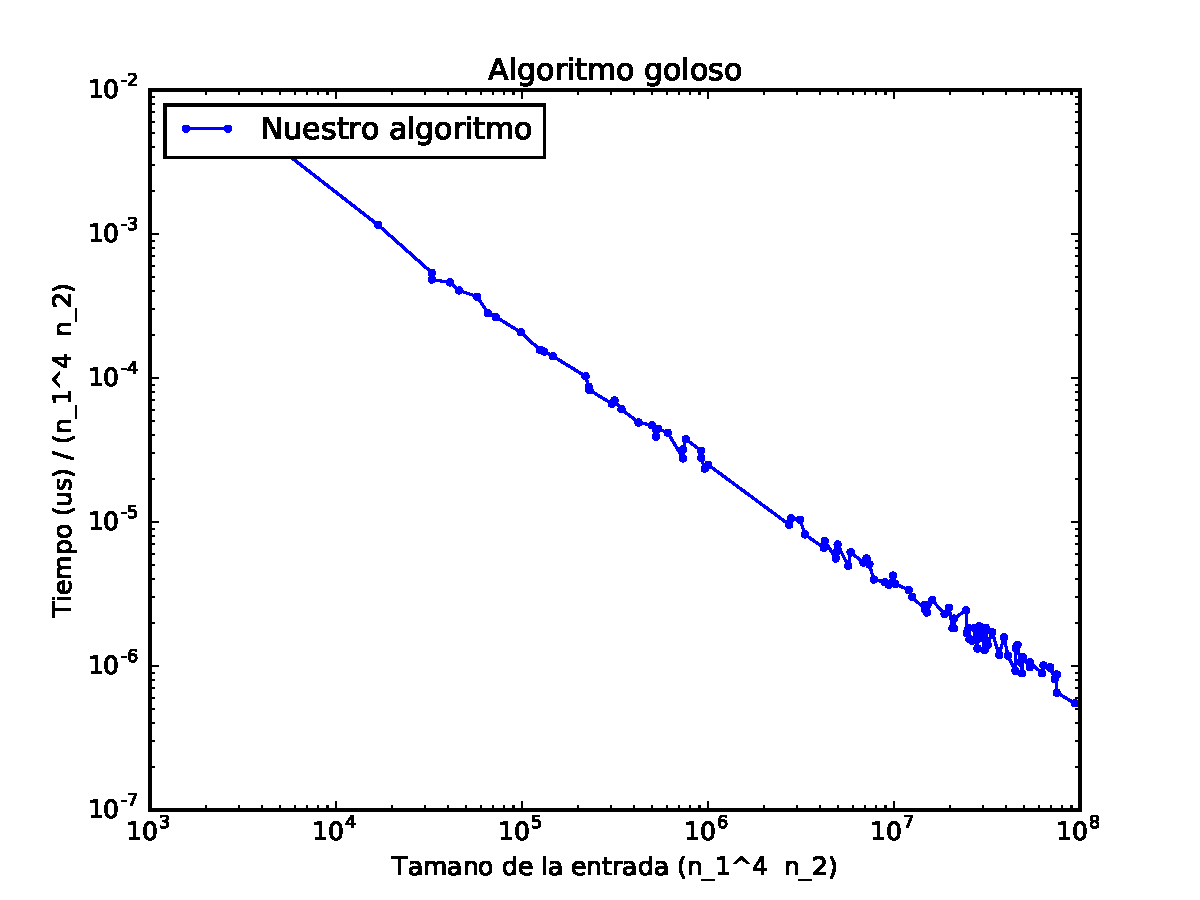
\includegraphics[width=0.9\textwidth]{graficos/problema_4/tiempos_1.pdf}
	\caption{}
	\label{fig:problema4-1}
\end{figure}

Se puede observar como, para instancias cada vez mas grandes, el tiempo en relación a la cota esperada decrece tendiendo a cero, de esto se puede deducir que nuestra cota no es la mas ajustada posible, o sea no serviría al mismo tiempo como cota inferior.

Como se puede observar, la complejidad que calculamos previamente depende de dos variables, $n_1$ y $n_2$, los siguientes gráficos analizan por separado que pasa cuando se varía cada uno de estos valores y se intenta corroborar que la complejidad es correcta.

\begin{figure}[H]
 \centering
	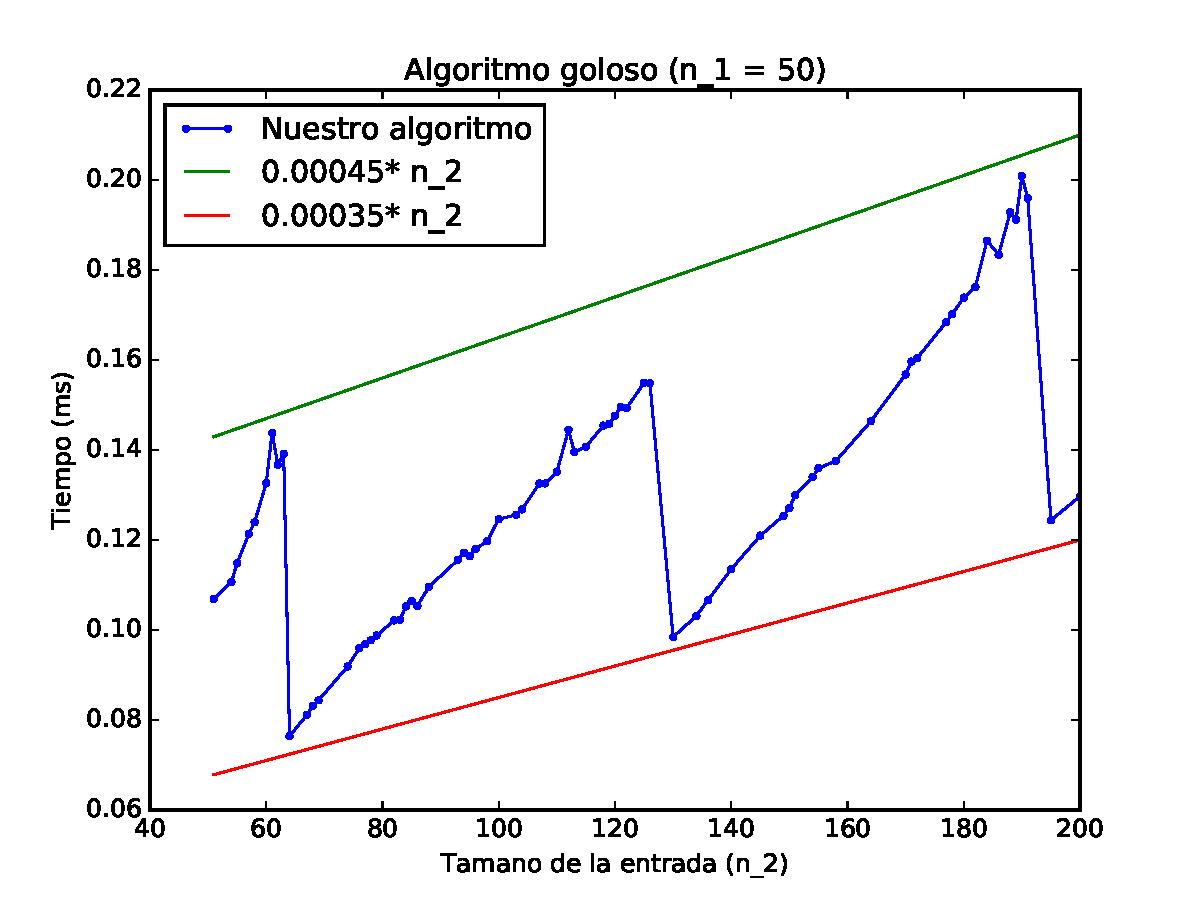
\includegraphics[width=0.9\textwidth]{graficos/problema_4/tiempos_2.pdf}
	\caption{}
	\label{fig:problema4-2}
\end{figure}

Este gráfico tiene dos particularidades que vale la pena comentar. Primero que púdimos ajustar el problema inferior y superiormente para esta variable. Segundo que hay picos, esto se debe a la manera en que maneja c++ a los vectores, estos se copian y aumentan de tamaño al pasar un tamaño multiplo de 64 elementos.

\begin{figure}[H]
 \centering
	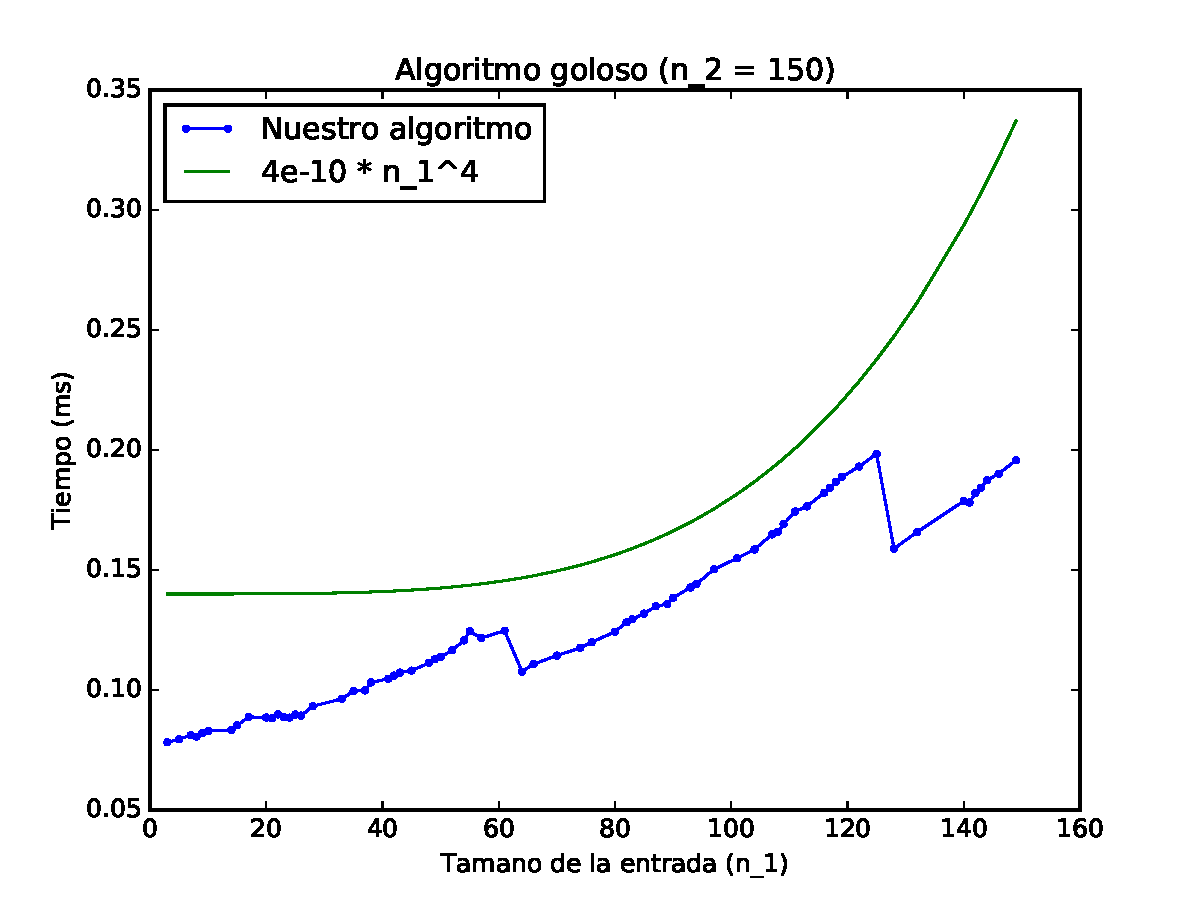
\includegraphics[width=0.9\textwidth]{graficos/problema_4/tiempos_3.pdf}
	\caption{}
	\label{fig:problema4-3}
\end{figure}

En este gráfico se ve como acotamos superiormente las instancias generadas con la complejidad que habiamos calculado, variando solo $n_1$.

La siguiente fígura expone la cantidad de aristas que tenian los isomorfismos calculados por nuestras dos heurísticas golosas, la mala (la primera) y la segunda, la que escogimos como nuestro algoritmo predilecto.

\begin{figure}[H]
 \centering
	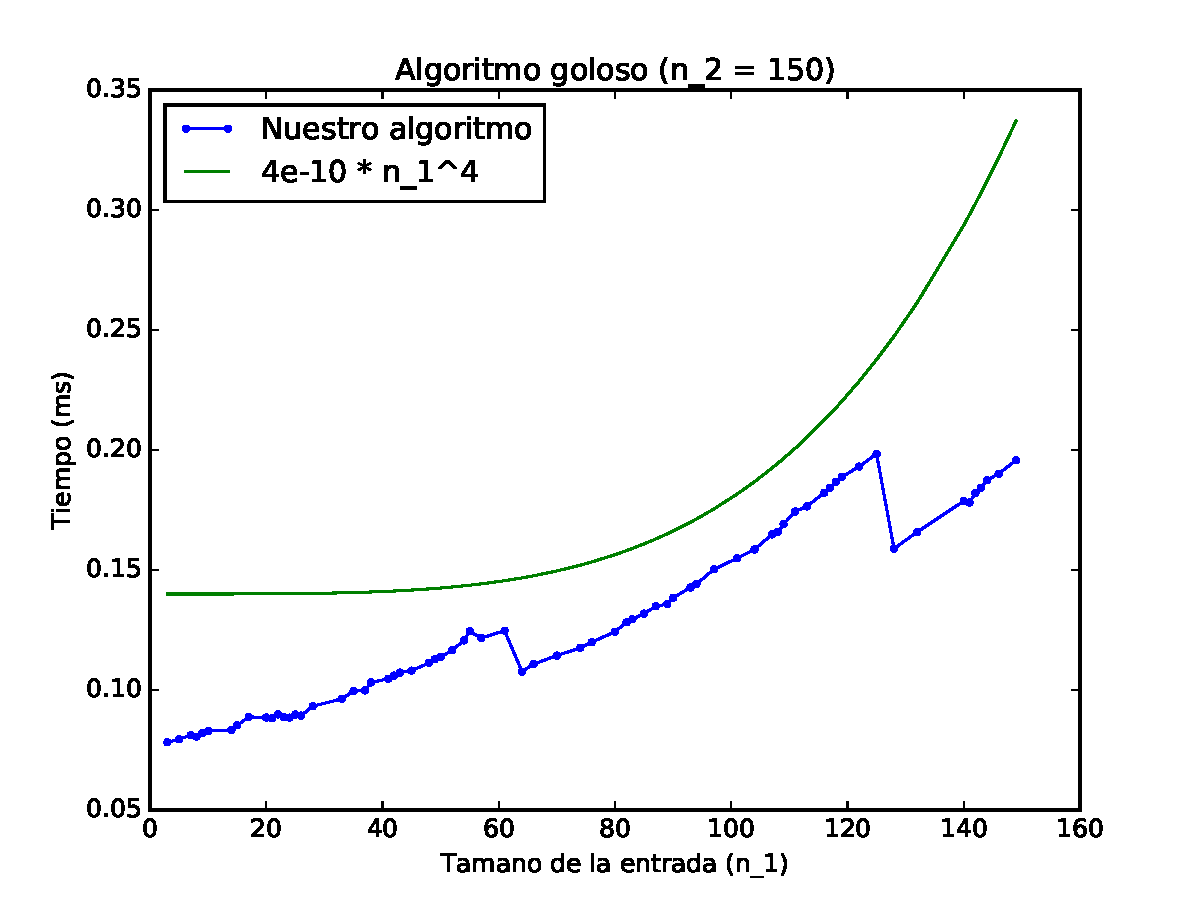
\includegraphics[width=0.9\textwidth]{graficos/problema_4/calidad.pdf}
	\caption{}
	\label{fig:problema4-4}
\end{figure}

Se puede ver como nuestro algoritmo siempre es en promedio superior en todos los casos. Aunque la ventaja no es  inmensa tampoco, lo cual deja a criterio de la aplicación deseada si es preferible usar una u otra, ya que si recordamos lo dicho antes, la complejidad del Goloso Malo es bastante mejor, $O(n_2^2)$.

\subsection{Método de experimentación}


\newpage


\section{Ejercicio 5}
\subsection{Introducción}
En la sección anterior implementamos y analizamos una heurística golosa para atacar el problema planteado. Si bien resulta bastante deseable desde el punto de vista de la complejidad temporal (polinomial de grado razonable), tiene el problema de que, como vimos, la solución que nos provee puede ser arbitrariamente mala y en el caso general no tenemos ningún tipo de garantía de qué tan cerca puede estar de una solución verdaderamente óptima.

Lo que quisiéramos entonces es poder refinar la solución que nos devuelve la heurística golosa para que se acerce más al máximo real. Para esto probaremos 3 algoritmos de búsqueda local. Dichos algoritmos se basan en la noción de ``vecindad'' de soluciones. Dada una solución fuente, una vecindad de $S$, $N(S)$, es un subconjunto del conjunto de posibles soluciones (en nuestro caso un subconjunto del conjunto de subgrafos comunes) que a diferencia de este último tiene un cardinal lo suficientemente pequeño como para poder ser recorrido en tiempo polinomial. Entonces los algoritmos de búsqueda local se diferenciarán a partir de la vecindad escogida en cada caso.

Es importante resaltar que los algoritmos de búsqueda local no dejan de ser algoritmos heurísticos cuya calidad dependerá tanto de la solución fuente utilizada como de la vecindad escogida. Los algoritmos solo nos garantizan que encontraremos el máximo de la vecindad (máximo local) que no necesariamente es el máximo global.

Otra cosa importante que también será común a todas las búsquedas es que cuando encontremos un máximo en la vecindad, si es mejor que la solución \emph{source}, no nos conformaremos con esto sino que pasaremos a explorar la vecindad correspondiente a esta nueva solución. De forma que se iterará la búsqueda hasta que se llegue a una solución que sea máxima en su vecindad.

En particular nosotros escogimos 3 vecindades para el problema, bajo los siguientes rótulos:
\begin{itemize}
	\item INTERCAMBIAR
	\item REEMPLAZAR
	\item 3-ROTACION 
\end{itemize}

En todos los casos la solución fuente inicial será la dada por el algoritmo goloso.

\subsection{Explicación detallada de los algoritmos}
En pos de la claridad separamos la explicación y el pseudocódigo de las tres vecindades. 

La notación usada será $n_1 = |V(G_1)|$, $n_2 = |V(G_2)|$, $m_1 = |E(G_1)|$ y $m_2 = |E(G_2)|$. Asumimos, por ser precondición para usar el algoritmo goloso y la heurística REMPLAZAR, que $n_1 \leq n_2$. 

\subsubsection{INTERCAMBIAR}
Un aspecto importante de nuestro algoritmo goloso es que siempre mapea exactamente todos los vértices del grafo con menor número de vértices a la hora de devolver la solución. En esta primera vecindad lo que planteamos es considerar todos los \emph{swapeos} posibles para el mapeo de la solución \emph{source}. Formalmente, si $S = \{(v_0, w_{i_1}),\hdots , (v_n, w_{i_n})\}$ es el mapeo de la solución \emph{source}, entonces la vecindad de tipo INTERCAMBIAR asociada a S es $N_I(S) = \{S' : S' = \{(v_0, w_{i_1}),\hdots , (v_p, w_{i_q}) , \hdots, (v_q, w_{i_p}), (v_n, w_{i_n})\}\}$.

\begin{algorithm}[H]
  \small
  \begin{algorithmic}[1]
  \caption{Pseudocódigo de INTERCAMBIAR}
  \label{algo:5-1}
    \Procedure{INT}{\texttt{Grafo} $G_1$, \texttt{set<int>} $vertices_1$, \texttt{Grafo} $G_2$, \texttt{set<int>} $vertices_2$}$\rightarrow$ \texttt{MCS}
      \State \texttt{MCS} $source \gets goloso(G_1, vertices_1, G_2, vertices_2)$
      \Comment $O()$
      \State \texttt{bool} $mejore \gets true$
      \Comment $O(1)$
      \While{$mejore$}
      \Comment $O(min\{m_1, m_2\})$
        \State $mejore \gets false$
        \Comment $O(1)$
        \For{$i \gets 0 \hdots |source.isomorfismo|$}
        \Comment $n_1$ veces
          \For{$j \gets 0\hdots |source.isomorfismo|, i \neq j$}
          \Comment $n_1$ veces
            \State $swap(source.isomorfismo[i].first, source.isomorfismo[j].first)$
            \Comment $O(1)$
            \State \texttt{int} $aristas \gets contar\_aristas\_isomorfismo(G_1, G_2, source.isomorfismo)$
            \Comment $O(n_1^2)$
            \If{$aristas > source.aristas$}
            \Comment $O(1)$
              \State $source.aristas \gets aristas$ 
              \Comment $O(1)$             
              \State $mejore \gets true$
              \Comment $O(1)$
            \EndIf
          \EndFor
        \EndFor
      \EndWhile
    \EndProcedure
  \end{algorithmic}
  Complejidad: $O(min{n_1, n_2})$
\end{algorithm}

\subsubsection{REEMPLAZAR}
Recordar que $n_1 \leq n_2$ por precondición. En particular, para esta vecindad solo nos interesarán los casos en que $n_1 < n_2$. Si ambos tamaños fueran iguales el algoritmo no modificará la solución golosa.

Debido a esta condición extra que asumimos sobre el tamaño de los grafos, para cualquier mapeo que tengamos como solución (en particular, el dado por el algoritmo goloso) siempre hay vértices de $G_2$ que no se están mapeando.

La motivación de esta vecindad entonces es ver qué sucede con la cantidad de aristas cuando en el mapeo de la solución fuente reemplazamos nodos de $G_2$ con otros que no habíamos usado originalmente.

Formalmente, si $S = \{(v_0, w_{1}),\hdots , (v_n, w_{n})\}$ es el mapeo de la solución fuente y $R = \{z_1, \hdots, z_r\}$ son los vértices de $G_2$ que no se mapearon en $S$, entonces \\
$N(S) = \{S': S' = S \textbackslash \{(v_i, w_i)\} \cup \{(v_i, z_i)\}\}$. 

\begin{algorithm}[H]
  \small
  \begin{algorithmic}[1]
  \caption{Pseudocódigo de REMPLAZAR}
  \label{algo:5-2}
    \Procedure{REMP}{\texttt{Grafo} $G_1$, \texttt{set<int>} $vertices_1$, \texttt{Grafo} $G_2$, \texttt{set<int>} $vertices_2$}$\rightarrow$ \texttt{MCS}
      \State \texttt{MCS} $source \gets goloso(G_1, vertices_1, G_2, vertices_2)$
      \State \texttt{bool} $mejore \gets true$
      \Comment $O(1)$
      \State \texttt{vector<int>} $vertices \gets set\_to\_vector(vertices_2)$
      \Comment $O(n_2-n_1)$
      \While{$mejore$}
      \Comment $O(min\{m_1, m_2\})$
        \State $mejore \gets false$
        \Comment $O(1)$
        \For{$i \gets 0 \hdots |vertices|$}
        \Comment $n_2-n_1$ veces
          \For{$j \gets 0 \hdots |source.isomorfismo|$}
          \Comment $n_1$ veces
            \State $swap(vertices[i], source.isomorfismo[j].second)$
            \Comment $O(1)$
            \State \texttt{int} $aristas \gets contar\_aristas\_isomorfismo(G_1, G_2, source.isomorfismo)$
            \Comment $O(n_1^2)$
            \If{$aristas > source.aristas$}
            \Comment $O(1)$
              \State $source.aristas \gets aristas$  
              \Comment $O(1)$            
              \State $mejore \gets true$
              \Comment $O(1)$
            \Else
              \State $swap(vertices[i], source.isomorfismo[j].second)$
              \Comment $O(1)$
            \EndIf
          \EndFor
        \EndFor
      \EndWhile
    \EndProcedure
  \end{algorithmic}
\end{algorithm}

\subsubsection{3-ROTACION}
Esta vecindad sigue un principio muy parecido al de INTERCAMBIAR. La idea surge por analogía de las búsquedas locales 2-opt y 3-opt vistas en la teórica. En INTERCAMBIAR solo considerábamos como vecindad las soluciones que estaban a un \emph{swap} de diferencia del mapeo fuente. En ese caso los \emph{swapeos} pueden considerarse como una rotación de solo dos elementos. En esta variación la vecindad estará compuesta por todas las soluciones que están a lo sumo a una rotación de 3 nodos de diferencia.

\begin{algorithm}[H]
  \small
  \begin{algorithmic}[1]
  \caption{Pseudocódigo de 3-ROTACION}
  \label{algo:5-3}
    \Procedure{3-ROT}{\texttt{Grafo} $G_1$, \texttt{set<int>} $vertices_1$, \texttt{Grafo} $G_2$, \texttt{set<int>} $vertices_2$}$\rightarrow$ \texttt{MCS}
      \State \texttt{MCS} $source \gets goloso(G_1, vertices_1, G_2, vertices_2)$
      \State \texttt{bool} $mejore \gets true$
      \Comment $O(1)$
      \While{$mejore$}
      \Comment $O(min\{m_1, m_2\})$
        \State $mejore \gets false$
        \Comment $O(1)$
        \For{$i \gets 0 \hdots |source.isomorfismo|$}
        \Comment $O(n_1)$ veces
          \For{$j \gets 0\hdots |source.isomorfismo|, i \neq j$}
          \Comment $n_1$ veces
            \For{$k \gets 0 \hdots |source.isomorfismo|$}
            \Comment $n_1$ veces
              \State $swap(source.isomorfismo[i].first, source.isomorfismo[k].first)$
              \Comment $O(1)$
              \State $swap(source.isomorfismo[k].first, source.isomorfismo[j].first)$
              \Comment $O(1)$
              \State \texttt{int} $aristas \gets contar\_aristas\_isomorfismo(G_1, G_2, source.isomorfismo)$
              \Comment $O(n_1^2)$
              \If{$aristas > source.aristas$}
              \Comment $O(1)$
                \State $source.aristas \gets aristas$ 
                \Comment $O(1)$             
                \State $source.isomorfismo \gets source.isomorfismo$
                \Comment $O(n_1)$
                \State $mejore \gets true$
                \Comment $O(1)$
              \EndIf
            \EndFor
          \EndFor
        \EndFor
      \EndWhile
    \EndProcedure
  \end{algorithmic}
\end{algorithm}

\subsection{Complejidades}
En este apartado se mantine la convención de que $n_1 = min\{n_1, n_2\}$.
Para calcular las complejidades en peor caso de las búsquedas tengamos en cuenta lo siguiente: en todos los casos se tiene por un lado el costo para recorrer completamente cada vecindad, y por el otro la cantidad de veces que vamos a tener que efectivamente vamos a tener que recorrer una vecindad. Esto último es debido a que, en peor caso, por cada mejora que logramos tenemos que recorrer una vecindad nueva. Calcular el costo de realizar cada recorrido es tan simple como ver los algoritmos de la subsección anterior y usar álgebra de órdenes. En cambio encontrar una cota no demasiado holgada para la cantidad de veces que se mejora no resulta trivial.

Por tales motivos primero desdoblaremos el cálculo del costo de cada iteración del de la cantidad de iteraciones.

\subsubsection{INTERCAMBIAR}
$O(n_1^4)$

\subsubsection{REMPLAZAR}
$O((n_2-n_1) n_1^3)$

\subsubsection{3-ROTACION}
$O(n_1^5)$

\subsubsection{Cantidad de iteraciones}
Para hallar una cota en peor caso para la cantidad de iteraciones (que vale para las tres vecindades) pensemos en la siguiente situación: la solución \emph{source} solo tiene una arista; además con cada iteración siempre mejoramos en solo una arista. Es claro que este es el peor escenario posible. También es relativamente fácil darse cuenta que la cantidad de iteraciones es $O(m_1)$, pues una solución máxima no puede tener más de $m_1$ aristas.

Es importante destacar que podría pasar que $G_2$ tenga menos aristas pero que las mismas usen más vértices de los que tiene $G_1$. Además si $m_2 < m_1$, $O(m_2) \subset O(m_1)$. Por eso está bien que sea $O(m_1)$ y no $O(min\{m_1, m_2\})$.

% Ahora bien no cuesta mucho darse cuenta en la práctica que esta cota puede ser realmente grosera por más de una razón: 
% \begin{itemize}
% \item por un lado asumimos una solución realmente mala: si bien en la sección respectiva vimos un ejemplo dónde la heurística se porta así de mal, no es esperable que en general de resultados tan malos;
% \item por otra parte asumimos que en cada iteración se mejora en exactamente un arista cuando la solución es $O(m_1)$. En general  
% \end{itemize}

En definitiva esta cota podría no ser alcanzable (nosotros no encontramos una instancia que la realice), pero seguro acota la cantidad de iteraciones y no pudimos encontrar una cota mejor en peor caso.

\subsection{Análisis de performance y calidad}

%%%%%Calidad%%%%%
\begin{figure}[H]
\centering
\begin{minipage}{0.49\textwidth}
  \centering
    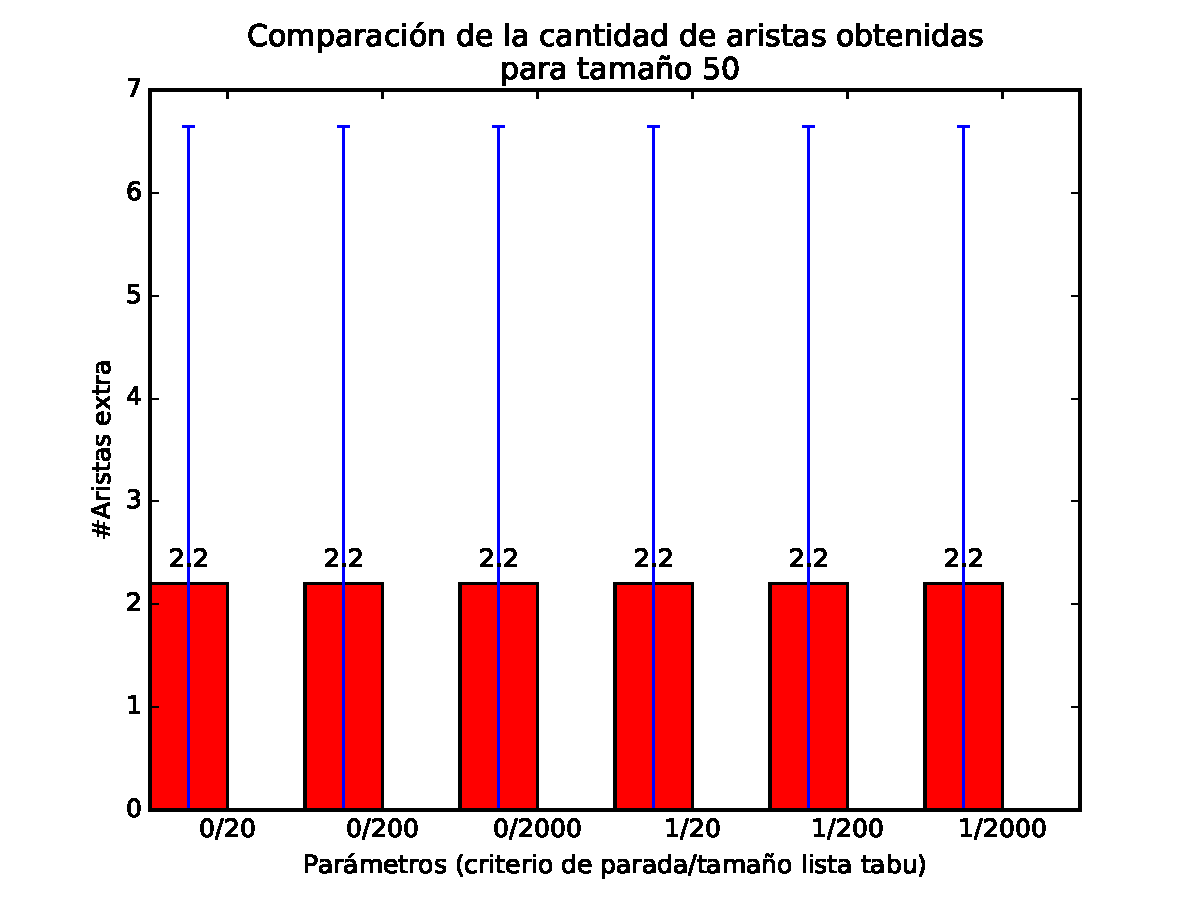
\includegraphics[width=1\textwidth]{graficos/problema_6/calidad0.pdf}
  \caption{\footnotesize{}}
  \label{fig:calidad5-1}
\end{minipage}%
\hspace{0.01\textwidth}
\begin{minipage}{0.49\textwidth}   
  \centering
    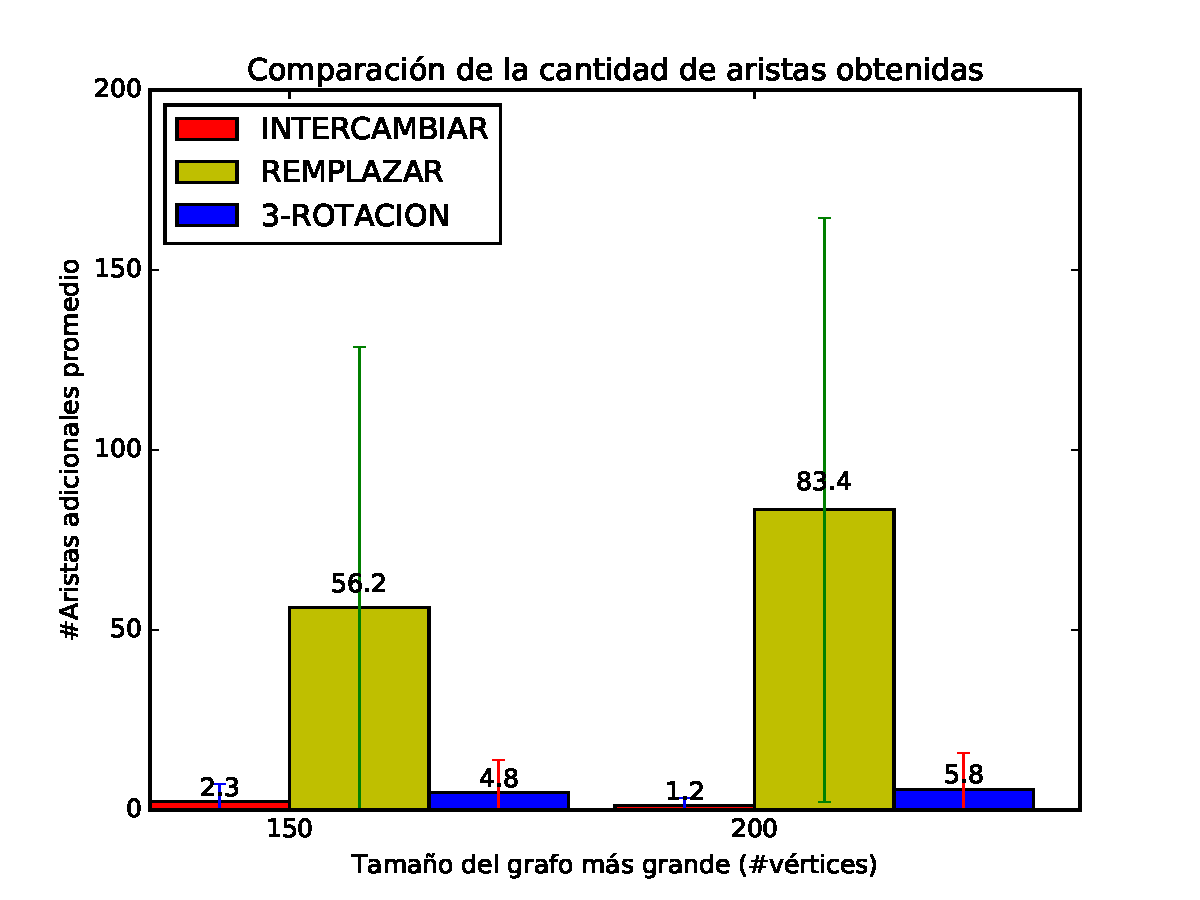
\includegraphics[width=1\textwidth]{graficos/problema_6/calidad2.pdf} 
  \caption{\footnotesize{}}
  \label{fig:calidad5-2}
\end{minipage}

\begin{minipage}{0.49\textwidth}
  \centering
    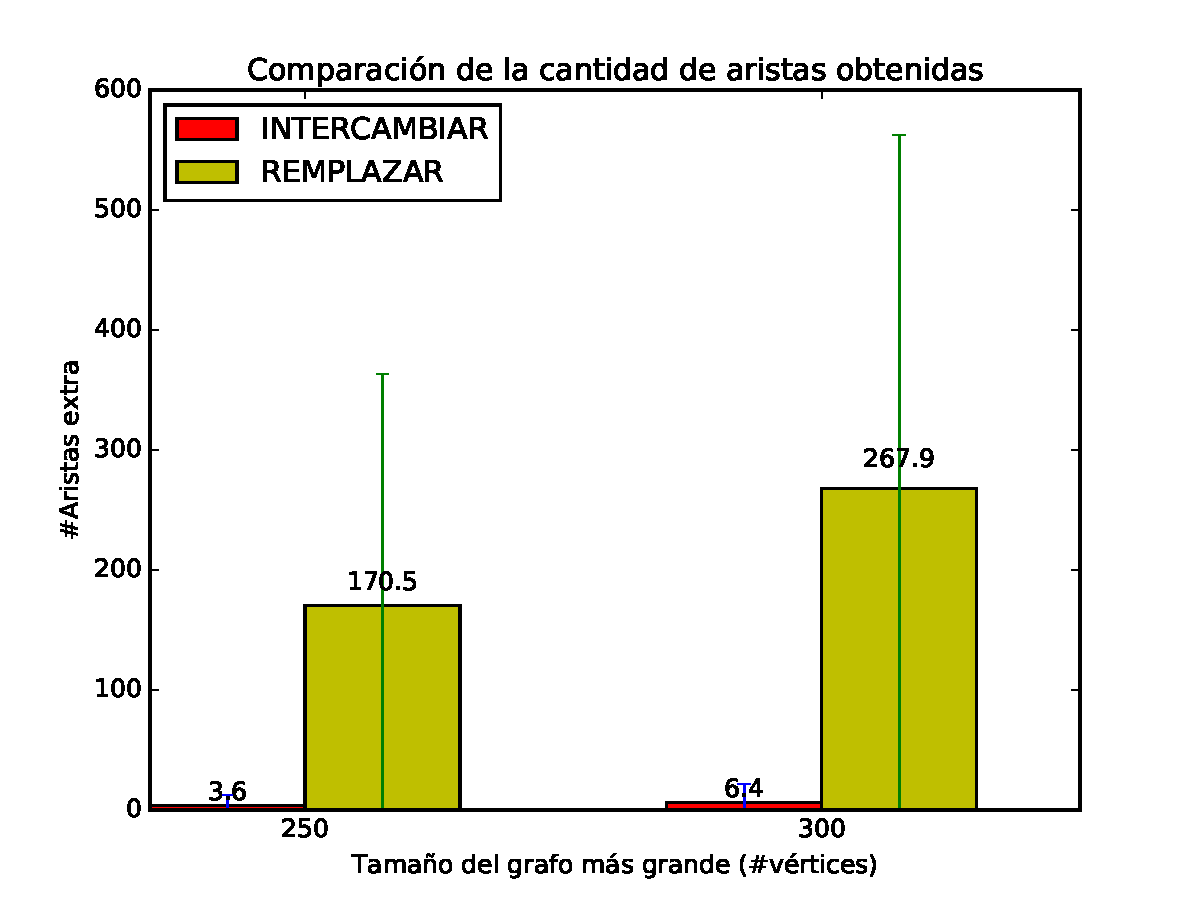
\includegraphics[width=1\textwidth]{graficos/problema_6/calidad4.pdf}
  \caption{\footnotesize{}}
  \label{fig:calidad5-3}
\end{minipage}%
\hspace{0.01\textwidth}
\begin{minipage}{0.49\textwidth}   
  \centering
    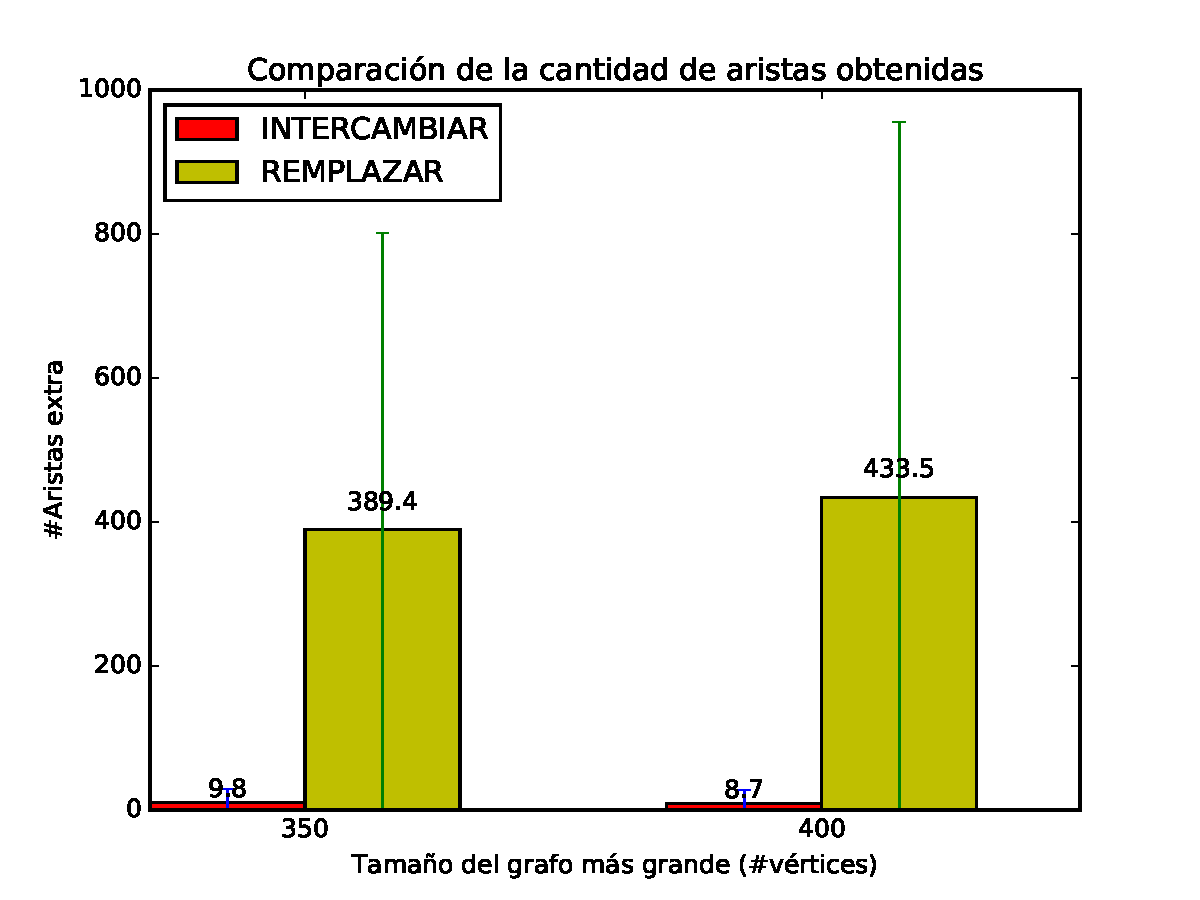
\includegraphics[width=1\textwidth]{graficos/problema_6/calidad6.pdf} 
  \caption{\footnotesize{}}
  \label{fig:calidad5-4}
\end{minipage}

\begin{minipage}{0.5\textwidth}   
  \centering
    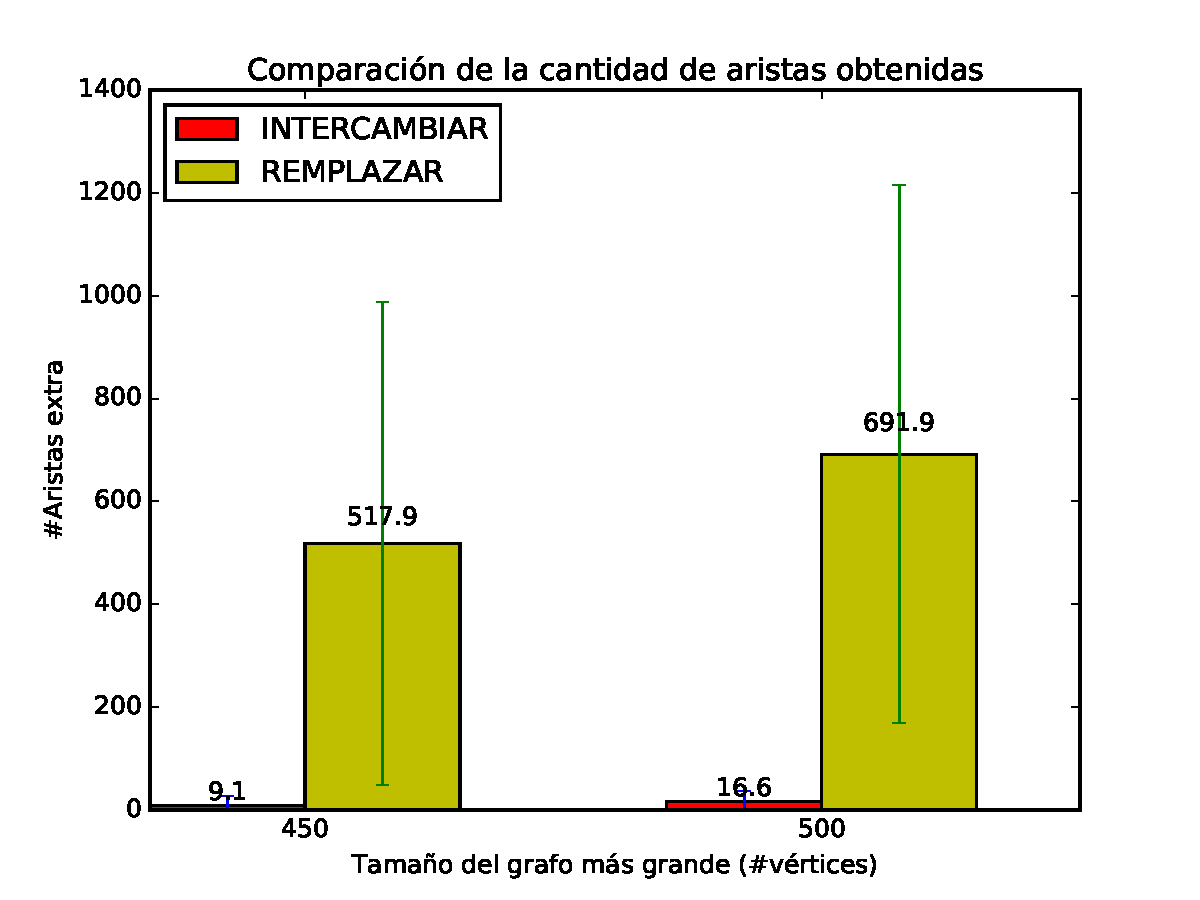
\includegraphics[width=1\textwidth]{graficos/problema_6/calidad8.pdf} 
  \caption{\footnotesize{}}
  \label{fig:calidad5-5}
\end{minipage}
\end{figure}


%%%%%Cociente%%%%%
\begin{figure}[H]
\centering
\begin{minipage}{0.49\textwidth}
  \centering
    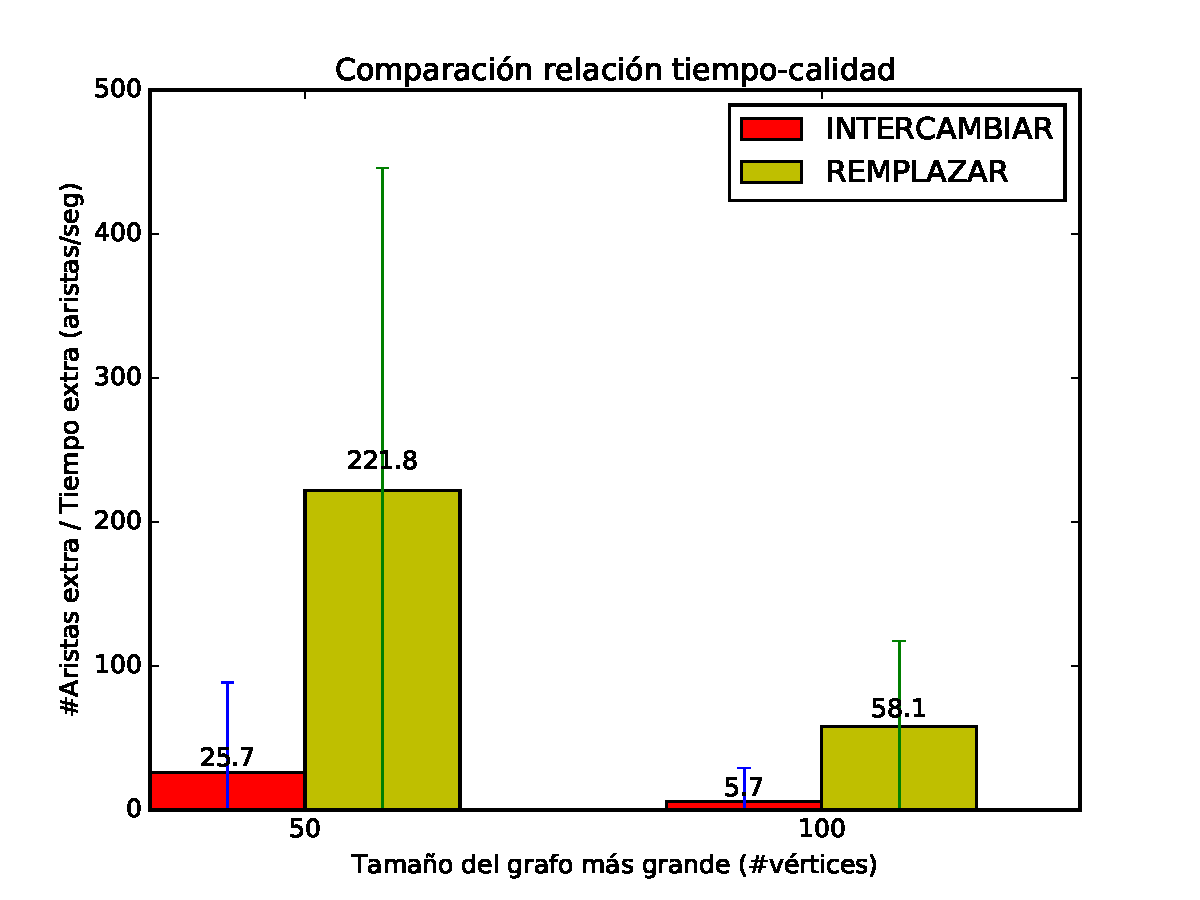
\includegraphics[width=1\textwidth]{graficos/problema_6/cociente0-0.pdf}
  \caption{\footnotesize{}}
  \label{fig:calidad5-1}
\end{minipage}%
\hspace{0.01\textwidth}
\begin{minipage}{0.49\textwidth}   
  \centering
    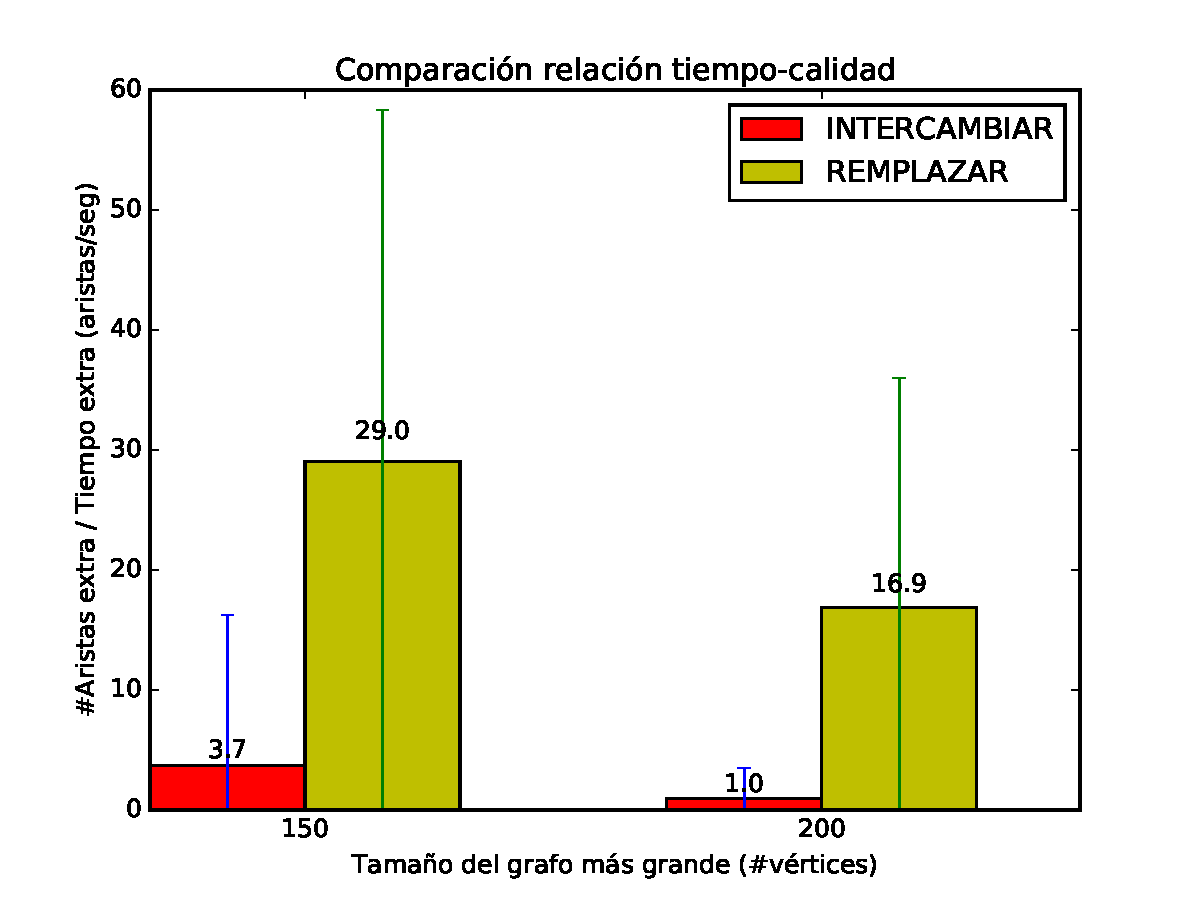
\includegraphics[width=1\textwidth]{graficos/problema_6/cociente0-2.pdf} 
  \caption{\footnotesize{}}
  \label{fig:calidad5-2}
\end{minipage}

\begin{minipage}{0.49\textwidth}
  \centering
    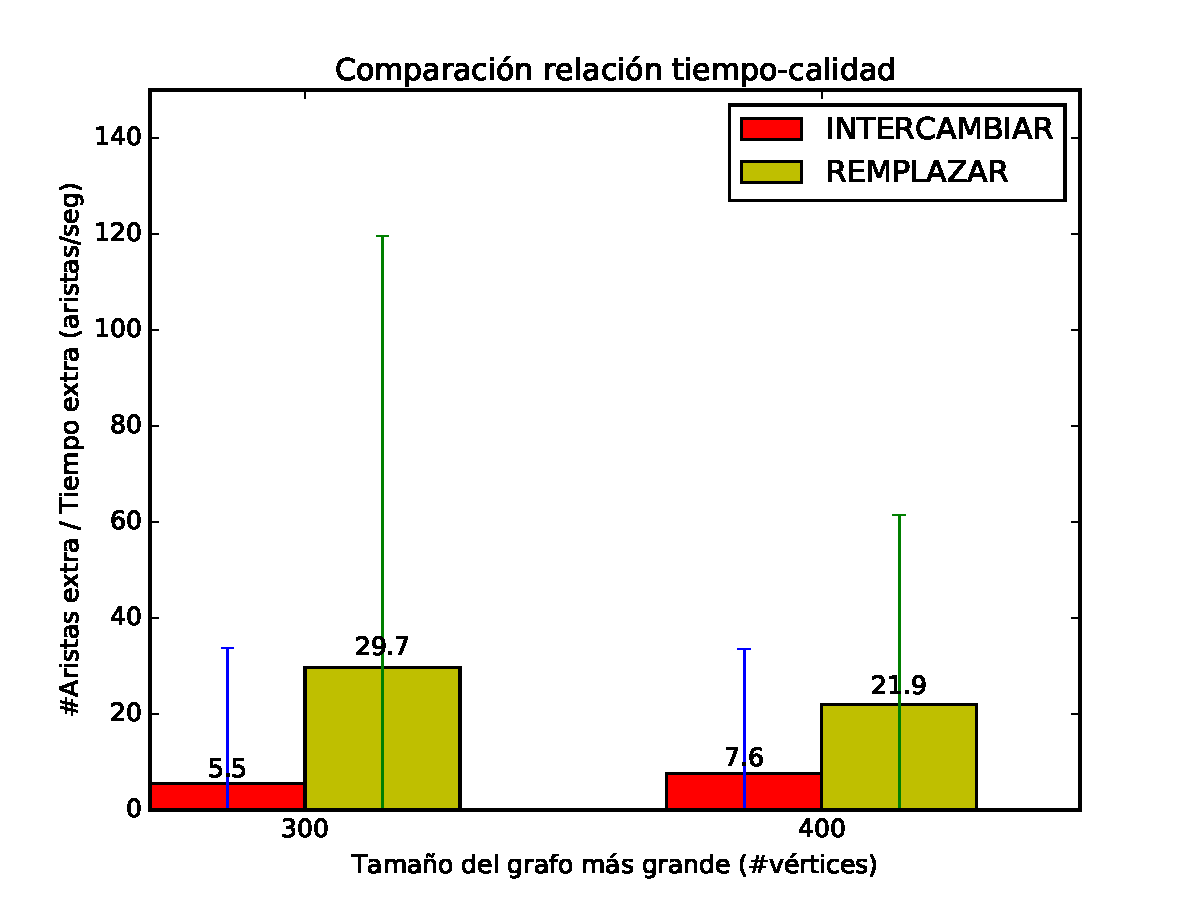
\includegraphics[width=1\textwidth]{graficos/problema_6/cociente0-4.pdf}
  \caption{\footnotesize{}}
  \label{fig:calidad5-3}
\end{minipage}%
\hspace{0.01\textwidth}
\begin{minipage}{0.49\textwidth}   
  \centering
    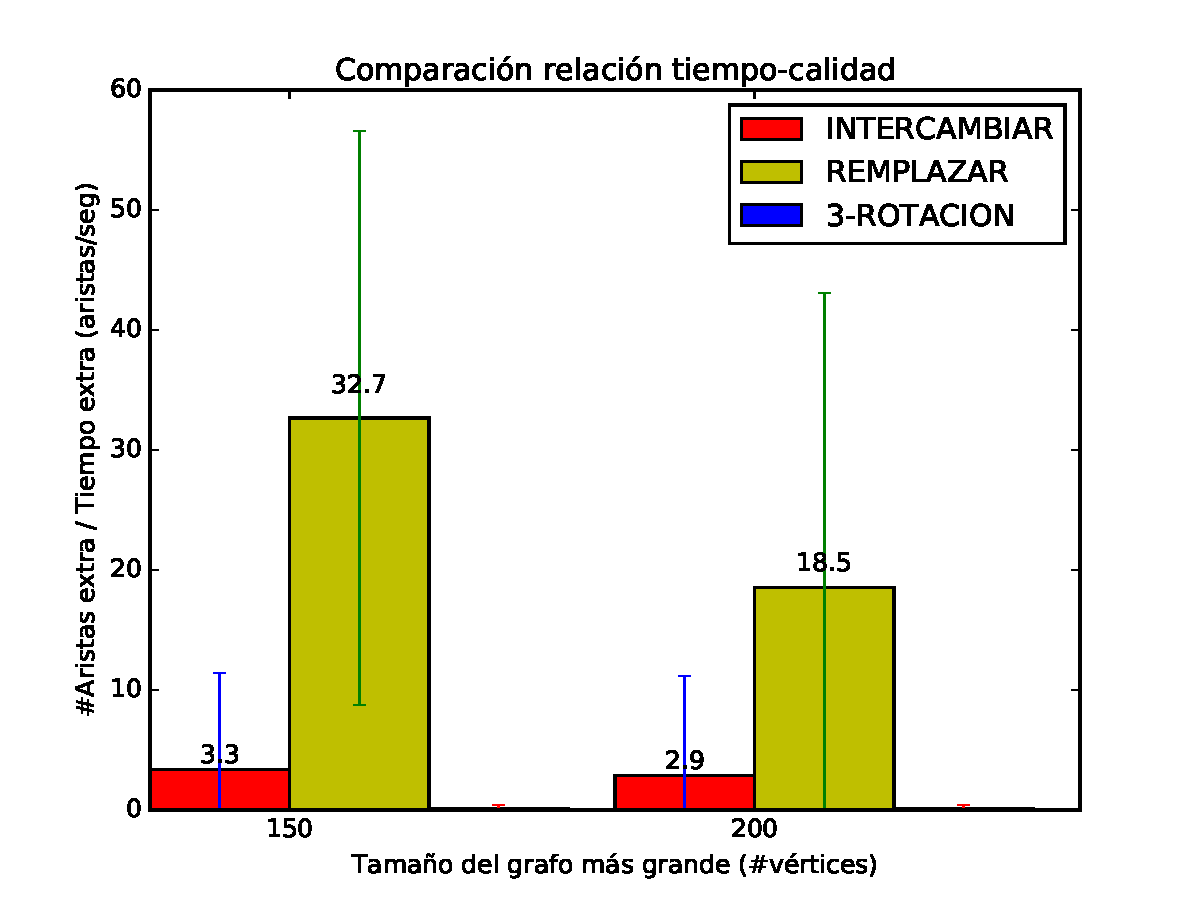
\includegraphics[width=1\textwidth]{graficos/problema_6/cociente1-2.pdf} 
  \caption{\footnotesize{}}
  \label{fig:calidad5-4}
\end{minipage}
\end{figure}


\begin{figure}[H]
  \centering
  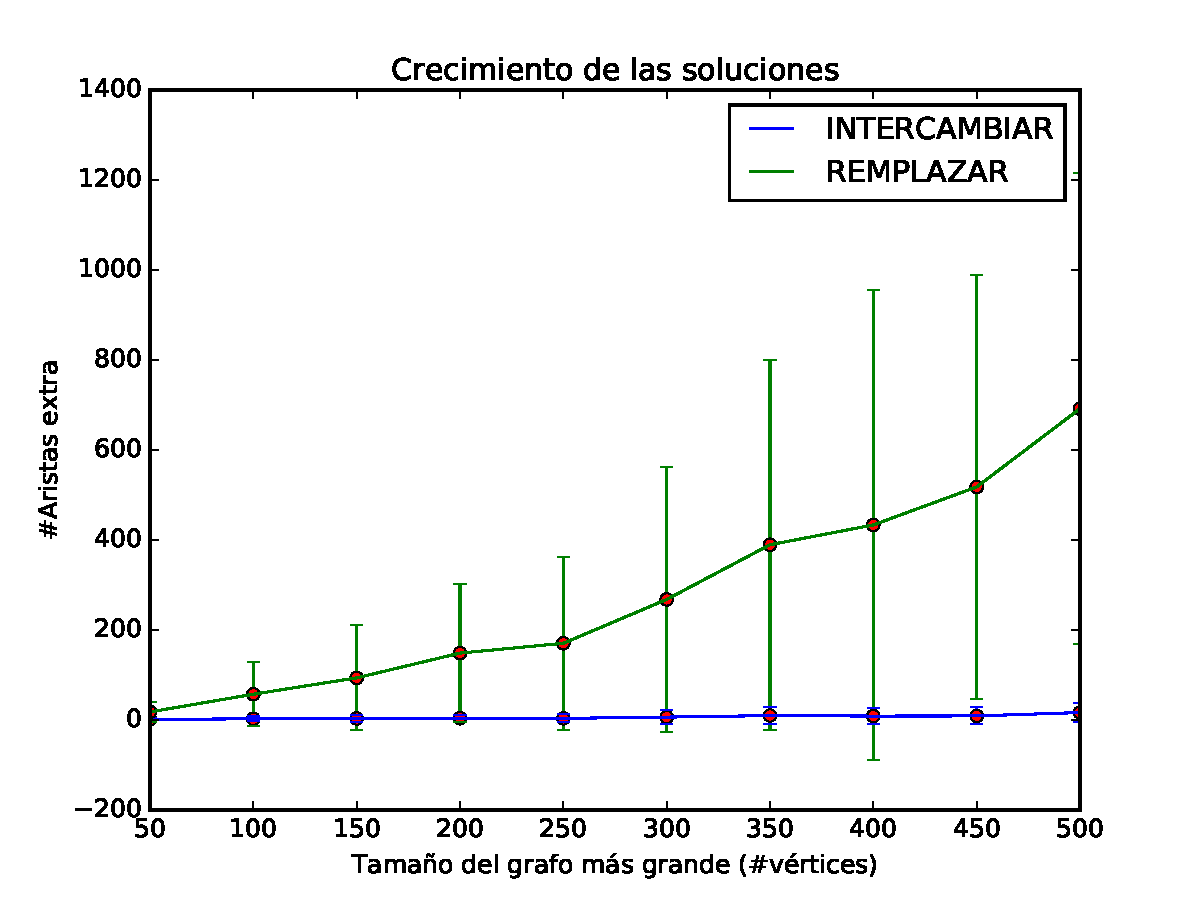
\includegraphics[width=1\textwidth]{graficos/problema_6/crecimiento.pdf} 
  \caption{\footnotesize{}}
  \label{fig:crecimiento}
\end{figure}
\newpage

\section{Ejercicio 6: Tabu Search}

\subsection{Explicación detallada del algoritmo}

En la sección anterior analizamos varios algoritmos de búsqueda local.
La búsqueda local es una heuristica para algoritmos aproximados.
Sin embargo, las heurísticas de búsqueda local pueden verse como un algoritmo de \emph{gradient descent}.
Estos algoritmos tienen el problema de los mínimos locales: cuando encuentran un mínimo local se quedan trabados y no pueden mejorar esa solución no óptima. 

Por esa razón surgen las metaheuristicas.
Una metaheurística es un método heurístico para resolver un  problema computacional general.
Una meteheurística usa los parámetros dados por el usuario sobre unos procedimientos genéricos y abstractos. 
Normalmente, estos procedimientos son heurísticos.

En particular, nosotros utilizaremos la metaheurística del tabu search, que a su vez se basa en la heurística de búsqueda local.




\subsection{Performance del algoritmo}


Para testear tanto este algoritmo como las heurísticas, utilizamos los casos cuya generación está explicada en el ap\'endice.

Antes de empezar con la explicación, debemos comentar que los tests de calidad y tiempos del tabú search son muy intensos computacionalmente: debían ser corridos por varias horas para que terminen.

Lo que presentamos es el resultado final, que aunque es el resultado de una sola corrida de varias horas, necesito algunas decenas de intentos anteriores, con el objetivo de encontrar los parámetros más interesantes a ser mostrados en el informe.

Por esa razón debimos limitar la cantidad de muestras que tomamos, lo cual, como vermos impactará un poco en las conclusiones que podremos obtener.
Sin embargo, los resultados son muy interesantes, y en el ejercicio 7 mostraremos algunos resultados que complementarán lo que no pudimos ver aquí.




En los gráficos, se verá que en el eje horizontal aparecen numeros de la pinta $n/m$.
$n$ será el criterio de parada utilizado, llamaremos 0 al criterio que cuenta la cantidad de iteraciones sin mejorar (el límite elegido será 500) y 1 al que harcodea el total de iteraciones (el límite elegido será 2000).
$m$ será el largo de la lista tabú.


Una aclaración importante es que probamos con distintos límites de iteraciones para cada criterio de parada y la diferencia en tiempo era la obvia (escalaba linealmente) y la diferencia en calidad era casi nula (a menos que las iteraciones fueran menores a 100. Por esa razón elegimos esas cantidades de iteraciones que nos parecieron lo suficientemente razonables.

No incluimos los gráficos de esos experimentos porque son mas que nada preliminares y no contribuyen a comparar las variantes, si no simplemente a optimizar los parámetros de cada una de ellas.



Primero analicemos la ``calidad'' de los algoritmos, es decir, que tan buenos son los resultados que devuelven. La métrica que utilizaremos es las aristas extra que devuelven, es decir, la cantidad de aristas que le agregan a la solución fuente, que es la de la heurística golosa.

Esta comparación será relativa: compararemos variantes del algoritmo unas contra otras, sin saber cual es la solución optima. Compararemos las soluciones del tabu search contra soluciones optimas en el ejercicio 7, aquí sólo nos atañe comparar las diferentes variantes de nuestro algoritmo.

Como dijimos anteriormente, la intensidad computacional de los algoritmos no permitió que podamos testear con grafos extremadamente grandes, utilizamos grafos de tamaño 150 como máximo. Sin embargo, 150 es un tamaño suficientemente grande, dado que ya a partir de 500, simplemente una corrida de un algoritmo comienza a tardar en el orden de 15 minutos: ni mencionar lo que se demora un test entero.

%% CALIDAD

\begin{figure}[H]
 \centering
	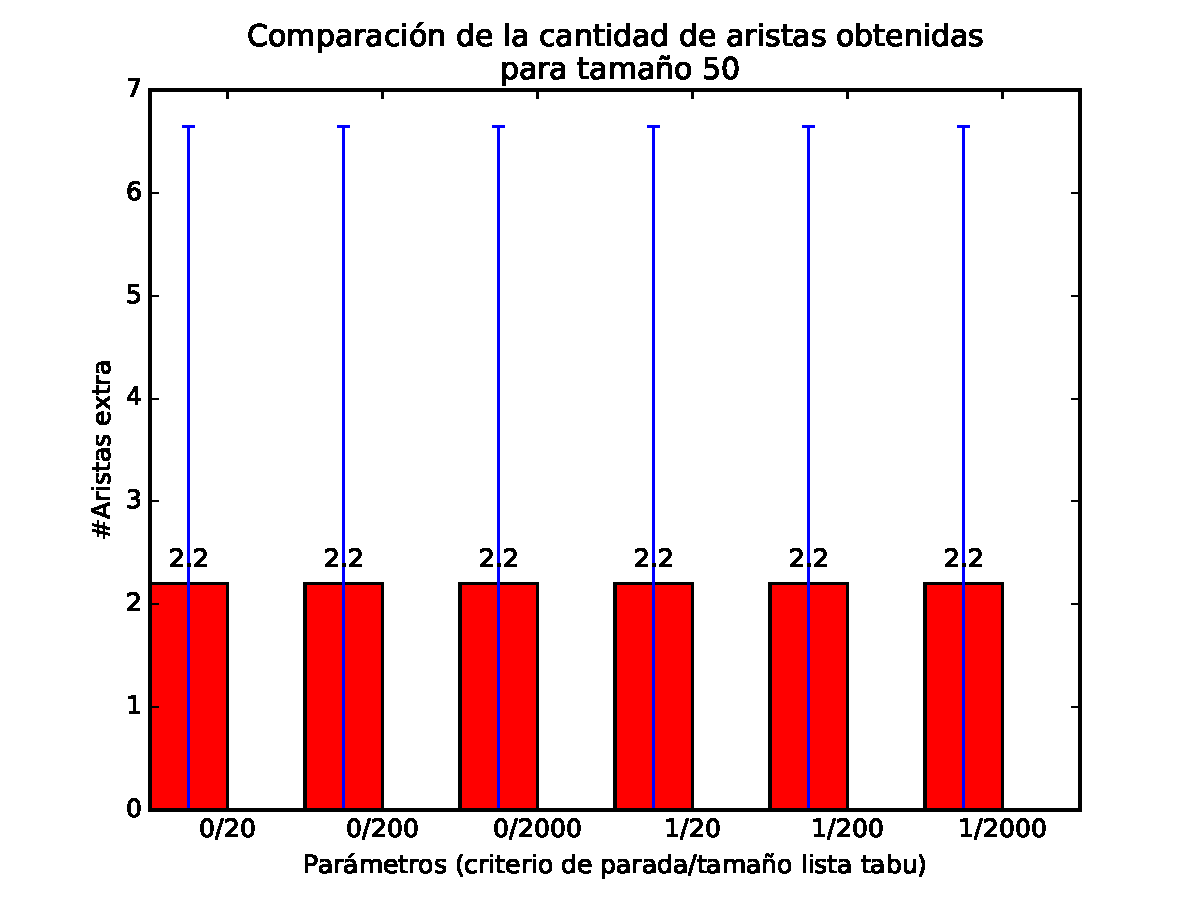
\includegraphics[width=0.8\textwidth]{graficos/problema_6/calidad0.pdf}
	\caption{}
	\label{fig:problema6-calidad0}
\end{figure}


\begin{figure}[H]
 \centering
	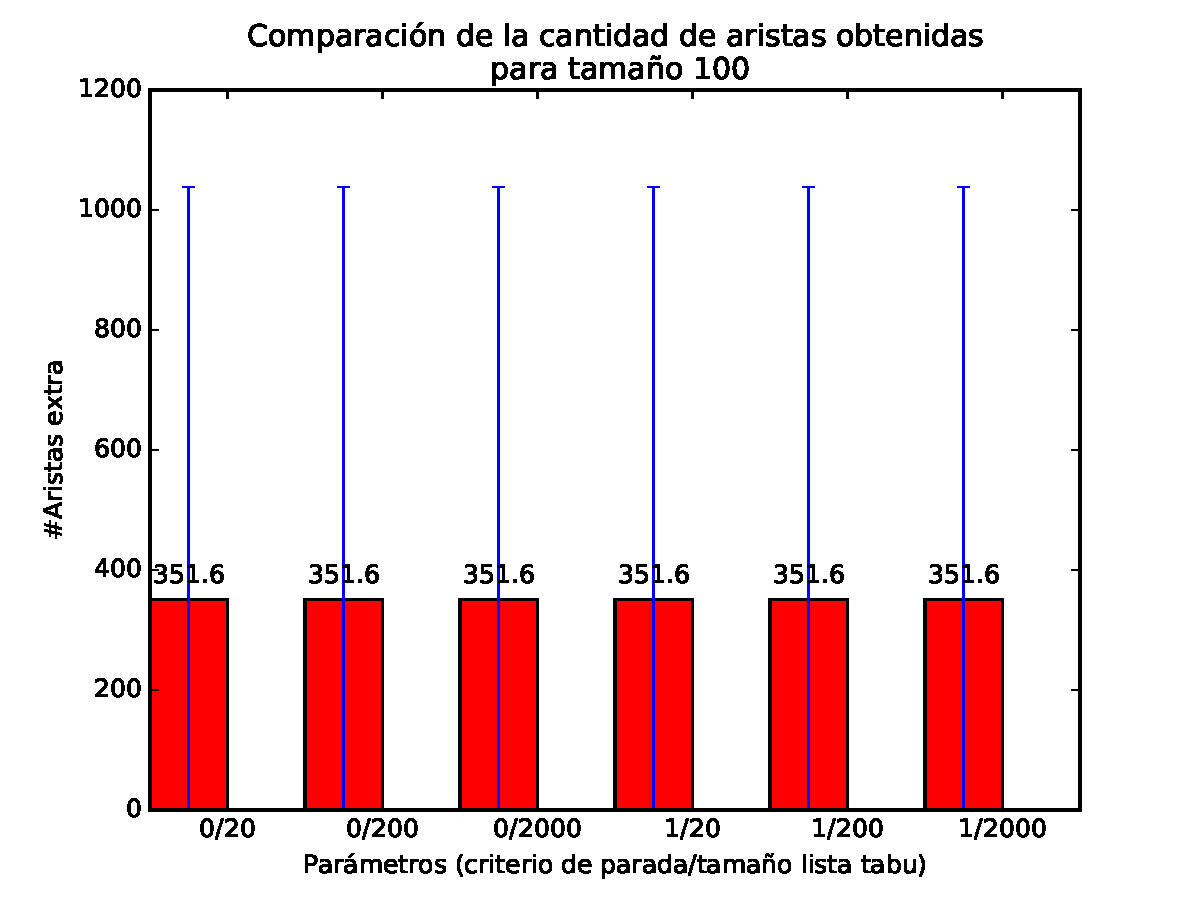
\includegraphics[width=0.8\textwidth]{graficos/problema_6/calidad1.pdf}
	\caption{}
	\label{fig:problema6-calidad1}
\end{figure}

\begin{figure}[H]
 \centering
	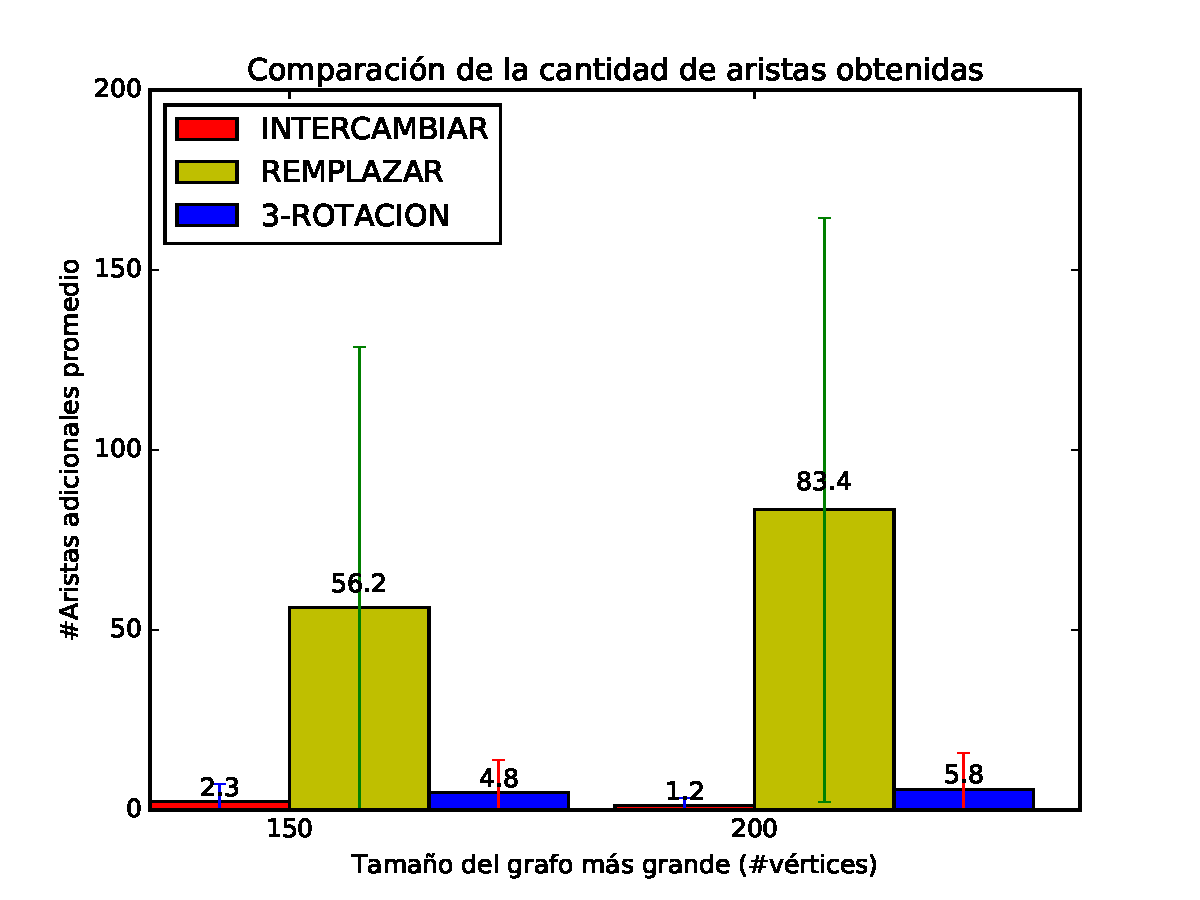
\includegraphics[width=0.8\textwidth]{graficos/problema_6/calidad2.pdf}
	\caption{}
	\label{fig:problema6-calidad2}
\end{figure}

En los gráficos se marca el promedio con una barra y la desviación estándar con un segmento.

Como podemos observar, no hay diferencia en el promedio de calidad de las mediciones.
Sin embargo, pudimos observar algunas diferencias en los máximos y los mínimos. Los mínimos de la variante que cuenta cuantas iteraciones no se mejoró eran mas altos.

Esto se debe a que el tamaño de los grafos no es lo suficientemente grande como para que dos algoritmos buenos hagan diferencia. Sin embargo, los grafos son lo suficientemente grandes como para asegurarnos que la diferencia entre las variantes no será demasiada en ningún caso (salvo casos patológicos).


A continuación, analizaremos los tiempos de los algoritmos. Nuestra expectativa, es que el tiempo que tarda la variante 0, es decir, la que fija la cantidad de iteraciones máxima sin que se mejore la solucion, va a ser mejor dado que optimiza la cantidad de iteraciones "ociosas", sobre todo en grafos chicos, donde la búsqueda se estanca relativamente rápido.

Además, esperamos que las variantes que tienen una lista tabú más larga tardan más, debido a que usamos una lista enlazada (std::list) para representarla, por lo que la búsqueda dentro de ella tiene complejidad lineal.

%% TIEMPOS
\begin{figure}[H]
 \centering
	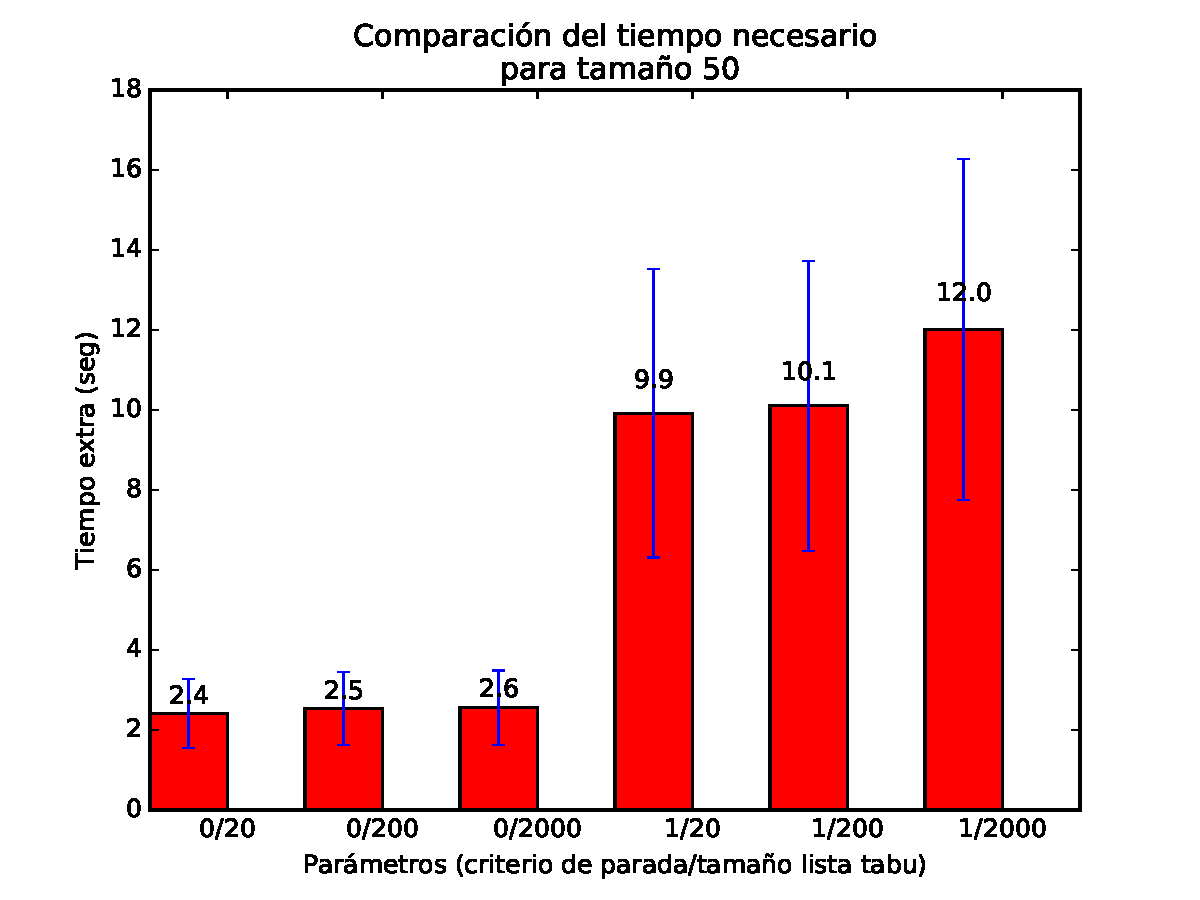
\includegraphics[width=0.8\textwidth]{graficos/problema_6/tiempo0.pdf}
	\caption{}
	\label{fig:problema6-tiempo0}
\end{figure}

\begin{figure}[H]
 \centering
	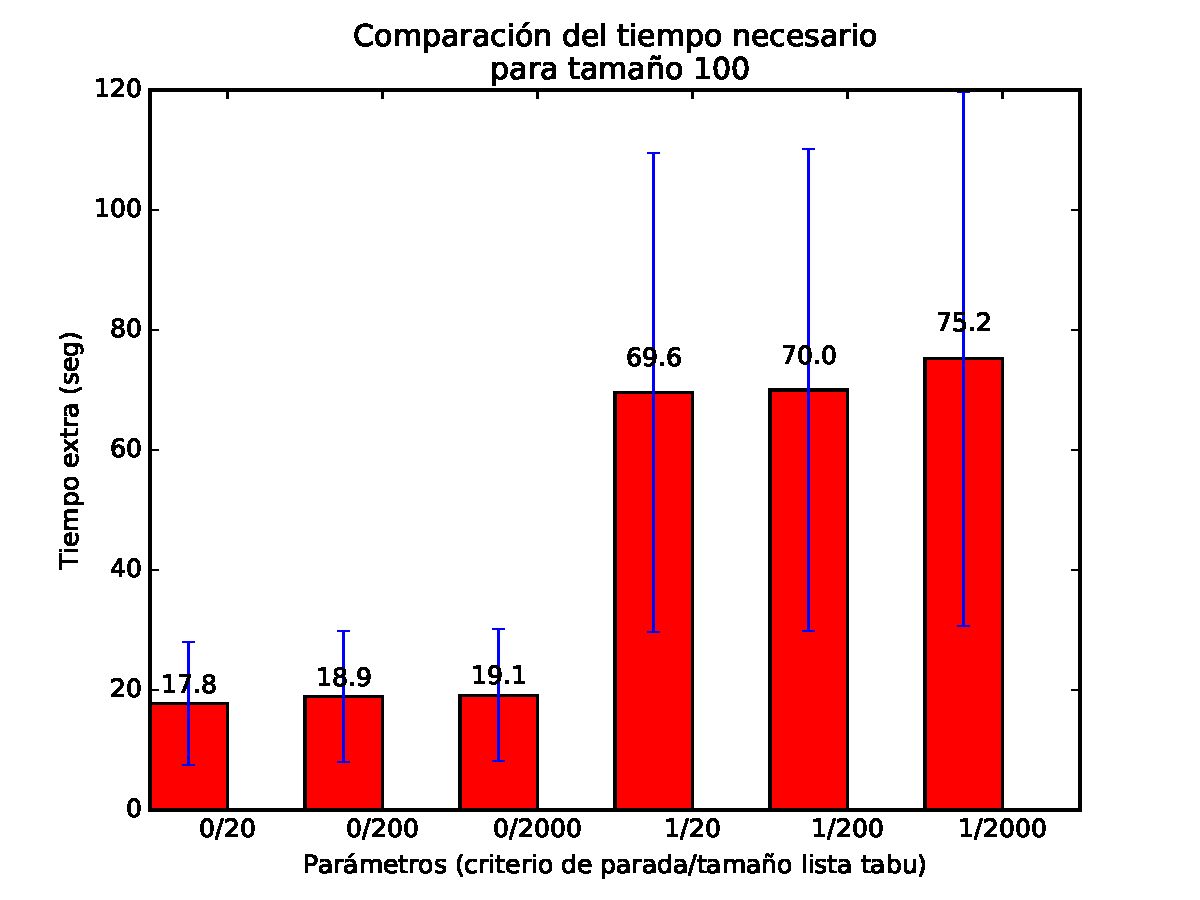
\includegraphics[width=0.8\textwidth]{graficos/problema_6/tiempo1.pdf}
	\caption{}
	\label{fig:problema6-tiempo1}
\end{figure}

\begin{figure}[H]
 \centering
	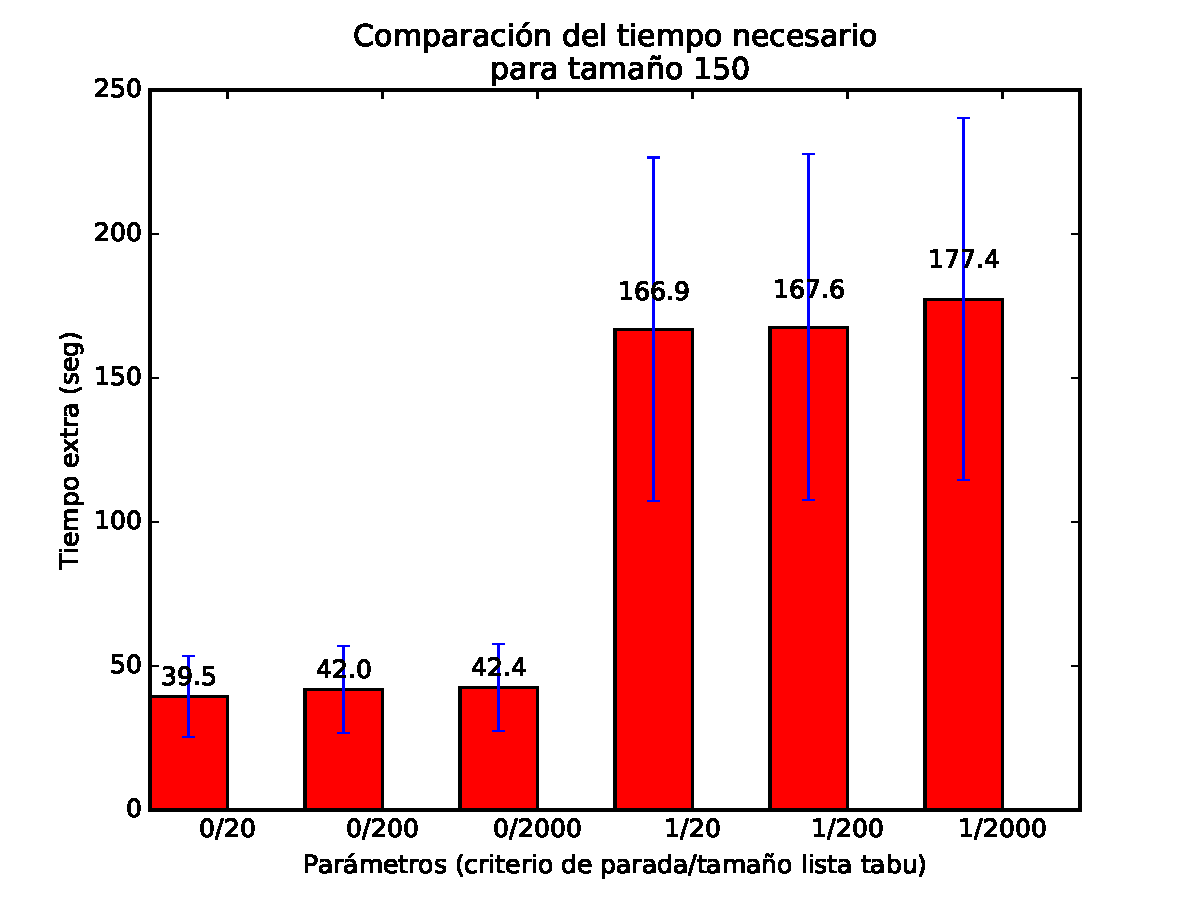
\includegraphics[width=0.8\textwidth]{graficos/problema_6/tiempo2.pdf}
	\caption{}
	\label{fig:problema6-tiempo2}
\end{figure}

En los gráficos se observa que confirmamos nuestras teorias de una manera bastante sólida.

Esto nos permite concluir que, aunque la calidad de las variantes es realmente similar, el tiempo que tardan los algoritmos es distinto, lo que nos permite concluir que la relación costo calidad de los algoritmos sí es diferente..

Esta relación costo calidad puede verse en los gráficos siguientes. En estos gráficos, dividimos la cantidad de aristas extra, sobre la el tiempo que tarda el algoritmo. Es decir, a más alto, mejor es el algoritmo.



%% COCIENTE

\begin{figure}[H]
 \centering
	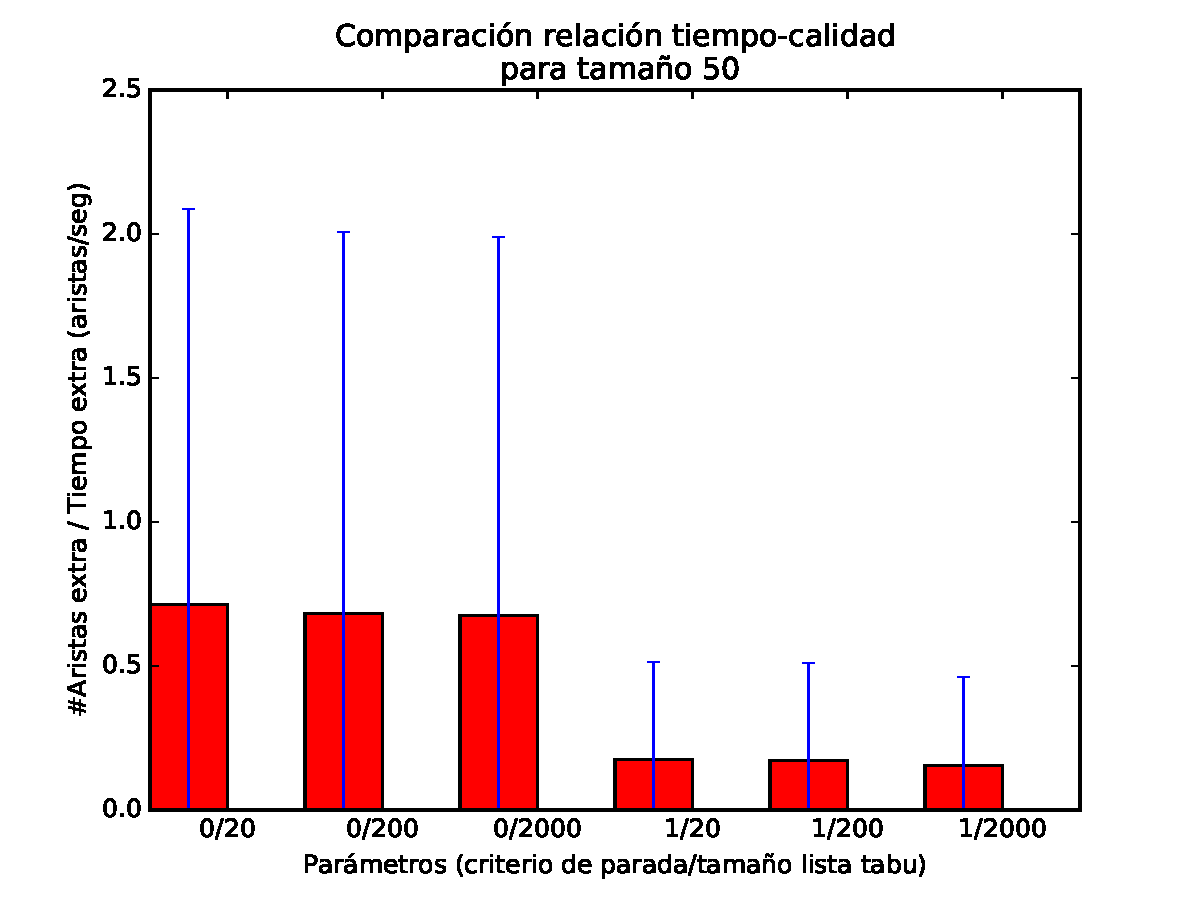
\includegraphics[width=0.8\textwidth]{graficos/problema_6/cociente0.pdf}
	\caption{}
	\label{fig:problema6-cociente0}
\end{figure}

\begin{figure}[H]
 \centering
	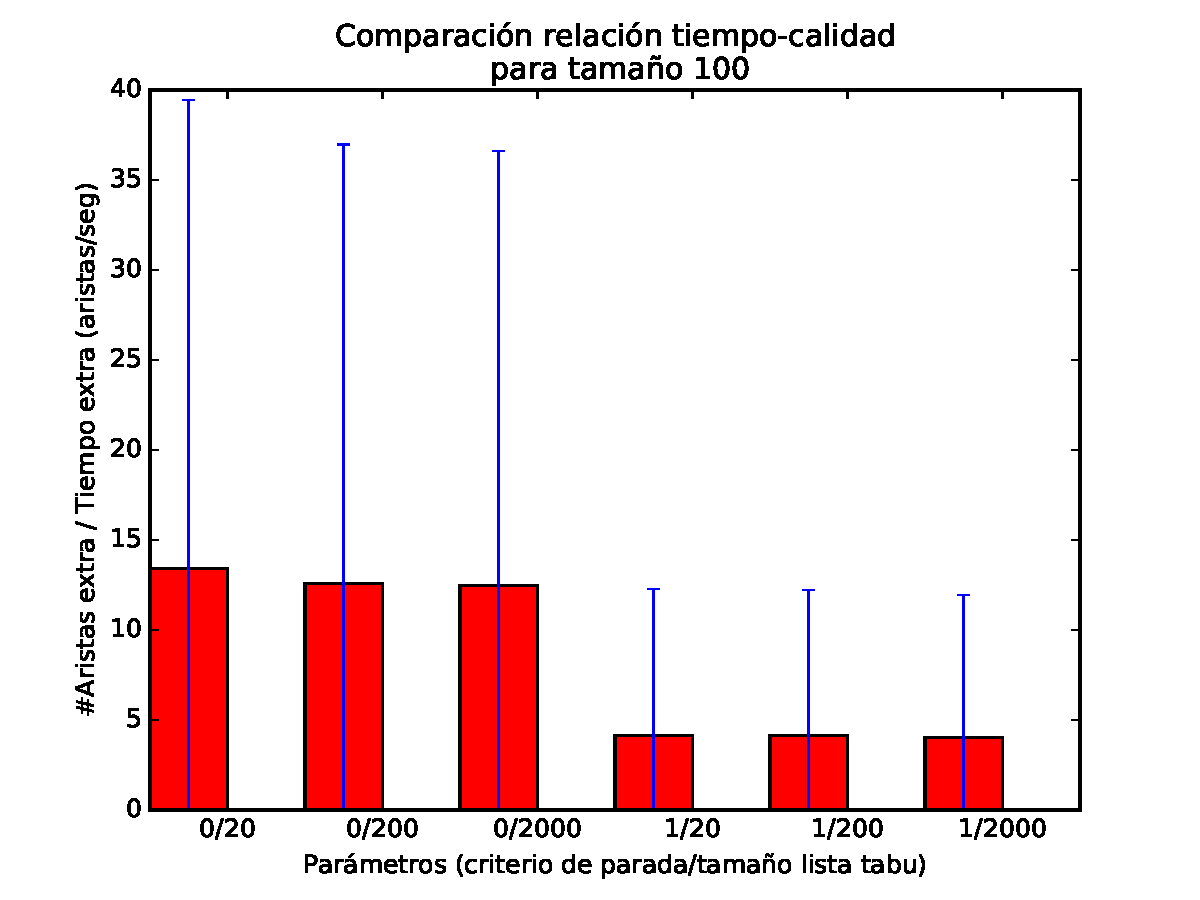
\includegraphics[width=0.8\textwidth]{graficos/problema_6/cociente1.pdf}
	\caption{}
	\label{fig:problema6-cociente1}
\end{figure}

\begin{figure}[H]
 \centering
	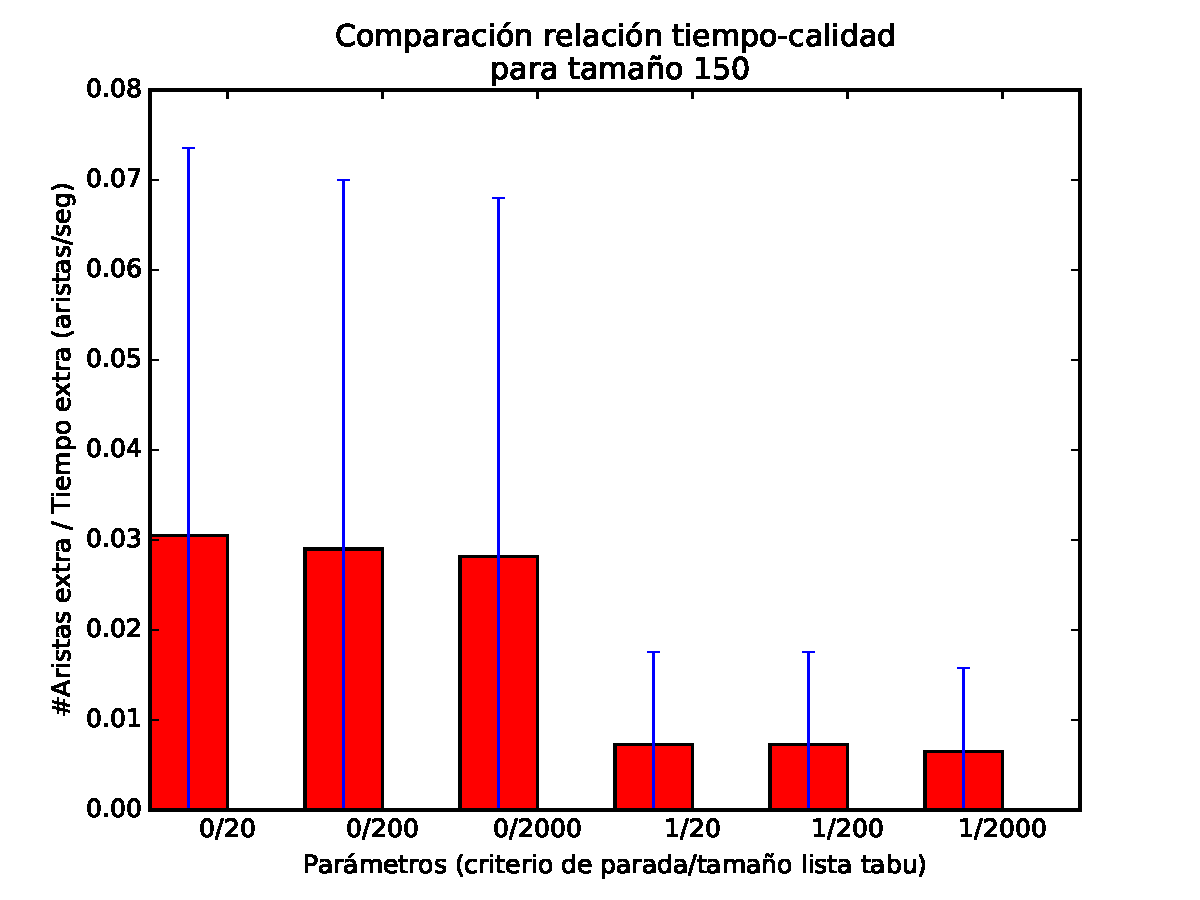
\includegraphics[width=0.8\textwidth]{graficos/problema_6/cociente2.pdf}
	\caption{}
	\label{fig:problema6-cociente2}
\end{figure}




\newpage

\section{Ejercicio 7}
El objetivo de esta sección será volver a experimentar, ahora que ya superamos una etapa de ajuste para las heurísticas, sobre un nuevo conjunto de instancias. También analizaremos las heurísticas y metaheurísticas en un caso cuya solución exacta conocemos de antemano. Finalmente, sacaremos en limpio algunas conclusiones sobre lo que fue la segunda parte de este trabajo, que consistió en probar diversas heurísticas. 

\subsection{Parámetros que elegimos}
Vamos a comparar la búsqueda local contra la búsqueda tabú. Para eso escogimos las configuraciones que nos resultaron más satisfactorias:
\begin{itemize}
	\item Para la búsqueda local escogimos INTERCAMBIAR, que mostraba tener una relación calidad-tiempo razonable.
	\item Para \emph{tabu search} escogimos el criterio de parada que espera a que hayan 500 iteraciones sin mejorar. En cuanto al tamaño de la lista tabú, en la medida que no había grandes diferencias, escogimos 200. Si bien con 20 era marginalmente más rápido y la calidad era la misma, pareciera que la mejora no es tanta como para sacrificar la robustez que puede brindar el tener una lista significativamente más larga.
\end{itemize}

Nuevamente, la comparación contra el algoritmo goloso se encuentra implícita pues tomamos las diferencias de aristas y tiempos con respecto a esta heurística.

\subsection{Resultados}
A continuación pasamos a presentar los resultados obtenidos para esta experimentación. A diferencia de otros experimentos como acá no hizo falta realizar muchas iteraciones de experimentación para ajustar cosas, se pudo tomar una muestra más significativa de instancias.

En las figuras de la \ref{fig:7-calidad1} a la \ref{fig:7-calidad3} se puede apreciar algo bastante esperable: \emph{tabu search} devuelve significativamente más aristas tanto en promedio como, más notoriamente, en los máximos. Sin embargo, algo muy destacable que no se aprecia directamente en los gráficos es que hubo algunos casos dónde la búsqueda local mejoró la solución golosa y la búsqueda tabú no. Esto es consistente con el hecho de que aunque sea una metaheurística de búsqueda global sigue sin tener garantías reales de encontrar un óptimo verdadero. Sin embargo, en los casos en los que esto ocurre la diferencia no es muy superior a una o dos aristas; mientras que en los casos que \emph{tabu search} es superior se pueden llegar a apreciar diferencias bastante más significativas.

Algo que fue transversal a toda la experimentación desde la sección 5 hasta aquí, aunque no fue mencionado antes, es que en general hay más casos donde los refinamientos no pudieron mejorar la solución que en los que sí se pudo. Además, en los casos en los que sí se mejoró generalmente la cantidad de aristas extras era poco significativa con respecto a la cantidad aristas que encontraba inicialmente el goloso\footnote{De hecho esta es quizás la razón más fuerte por la que graficamos diferencias y no los valores en crudo, pues notar la superioridad de un algoritmo u otro hubiese resultado complicado. También el hecho de que hayan muchos casos donde la diferencia es 0 produce que en general los gráficos de calidad que vimos tengan en genral barras bastante bajas con varianzas muy altas.}. Estos no son detalles menores pues nos hablan de que la calidad de las soluciones provistas por la heurística golosa es generalmente bastante alta \emph{per se}, o bien que simplemente son difíciles de mejorar. Un dato a tener en cuenta.
 
\begin{figure}[H]
\centering
\begin{minipage}{0.49\textwidth}
  \centering
    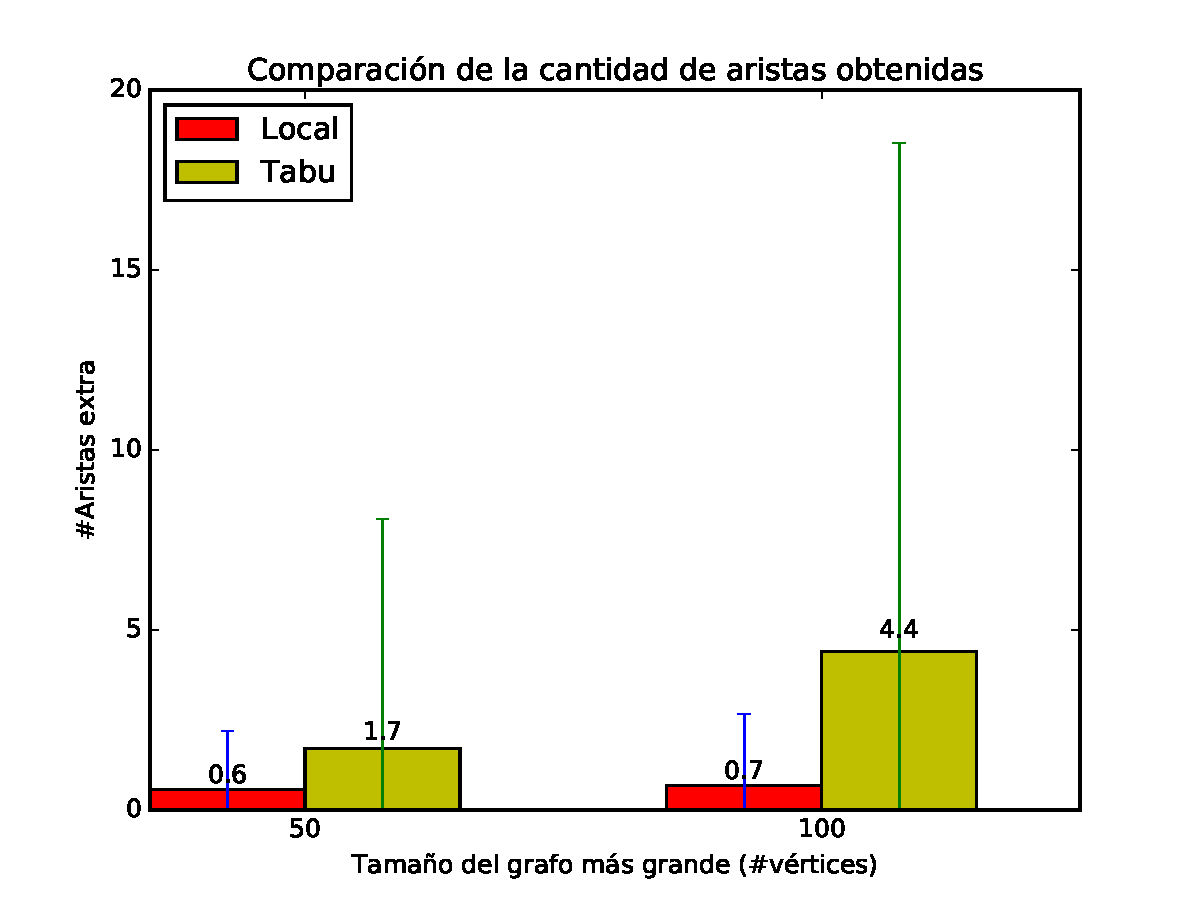
\includegraphics[width=1\textwidth]{graficos/problema_7/calidad0.pdf}
  \caption{}
  \label{fig:7-calidad1}
\end{minipage}%
\hspace{0.01\textwidth}
\begin{minipage}{0.49\textwidth}   
  \centering
    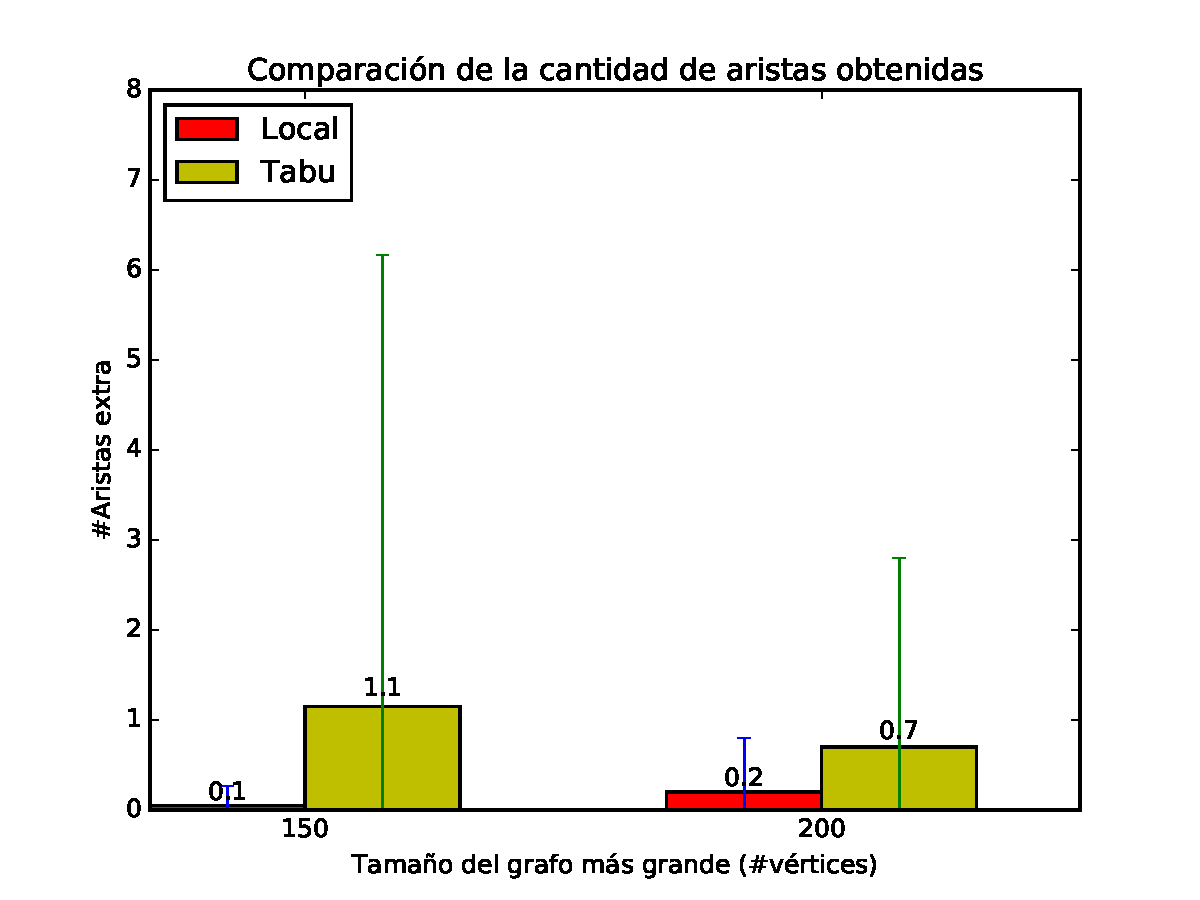
\includegraphics[width=1\textwidth]{graficos/problema_7/calidad2.pdf} 
  \caption{}
  \label{fig:7-calidad2}
\end{minipage}

\begin{minipage}{0.49\textwidth}
  \centering
    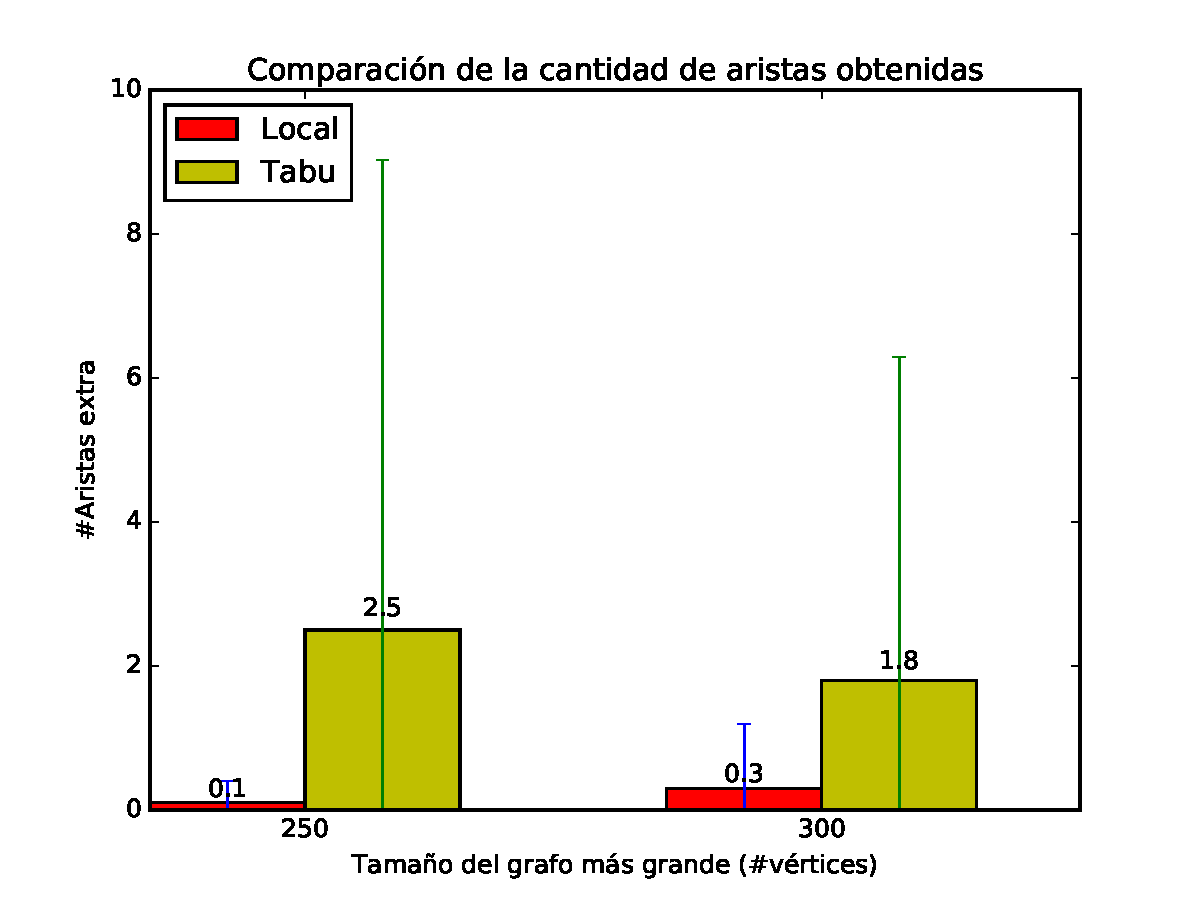
\includegraphics[width=1\textwidth]{graficos/problema_7/calidad4.pdf}
  \caption{}
  \label{fig:7-calidad3}
\end{minipage}%
\end{figure}

En las figuras de la \ref{fig:7-tiempo1} a la \ref{fig:7-tiempo3} se comparan los tiempos de ejecución. La diferencia es abrumadora en favor de la búsqueda local. No hay mucho más para decir al respecto pues en definitiva era esperable, aunque sí resulta sorprendente una diferencia tan abultada. 

Finalmente en las figuras \ref{fig:7-cociente1} a \ref{fig:7-cociente3} vemos los gráficos para la relación calidad/tiempo. Resulta claro al ver esot que dicha relación está dominada por el tiempo más que por la calidad (algo parecida ocurría en la sección 5, aunque aquí resulta más evidente). Un detalle a destacar es que aunque en general siempre usamos segundos como medida del tiempo, en este caso concreto tuvimos que usar minutos de forma que fuese apreciable el valor para la metaheurística.

\begin{figure}[H]
\centering
\begin{minipage}{0.49\textwidth}
  \centering
    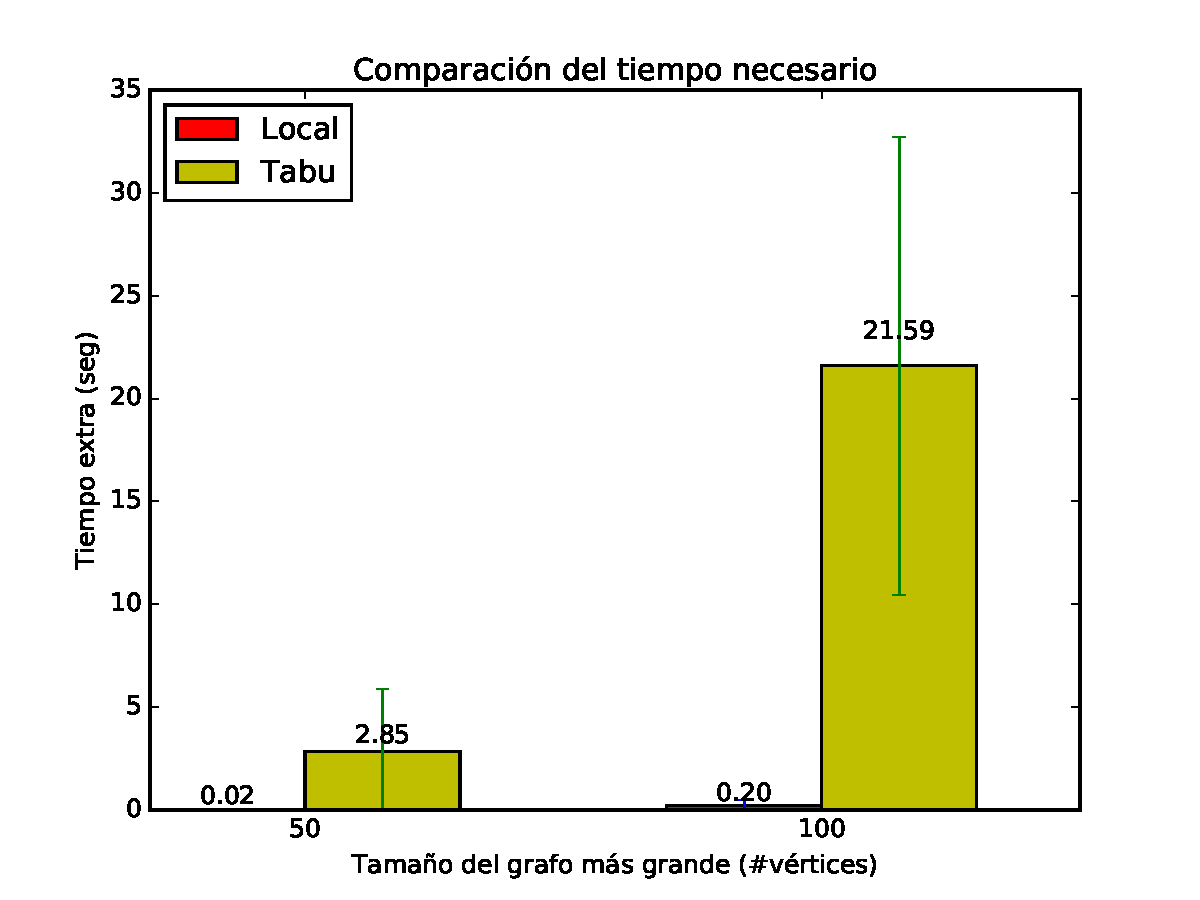
\includegraphics[width=1\textwidth]{graficos/problema_7/tiempo0.pdf}
  \caption{}
  \label{fig:7-tiempo1}
\end{minipage}%
\hspace{0.01\textwidth}
\begin{minipage}{0.49\textwidth}   
  \centering
    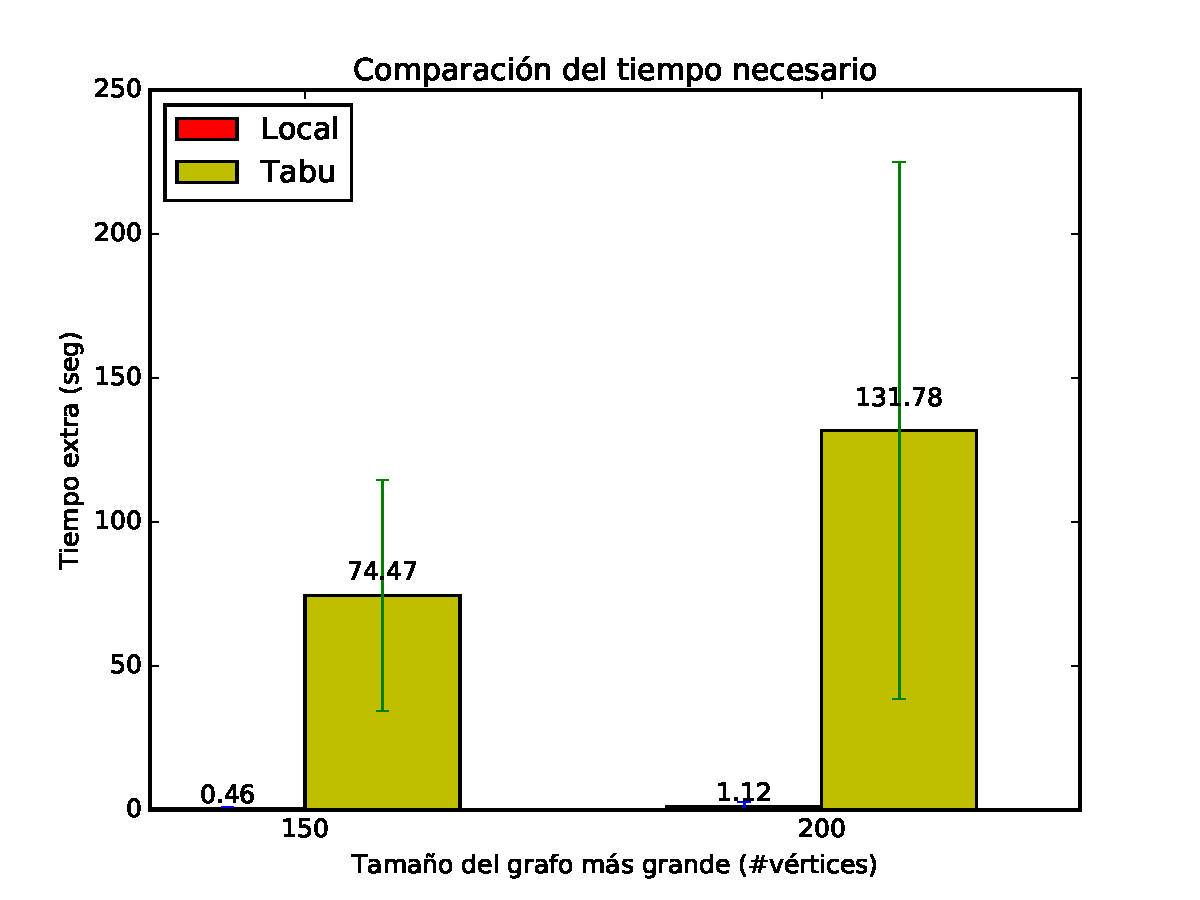
\includegraphics[width=1\textwidth]{graficos/problema_7/tiempo2.pdf} 
  \caption{}
  \label{fig:7-tiempo2}
\end{minipage}

\begin{minipage}{0.49\textwidth}
  \centering
    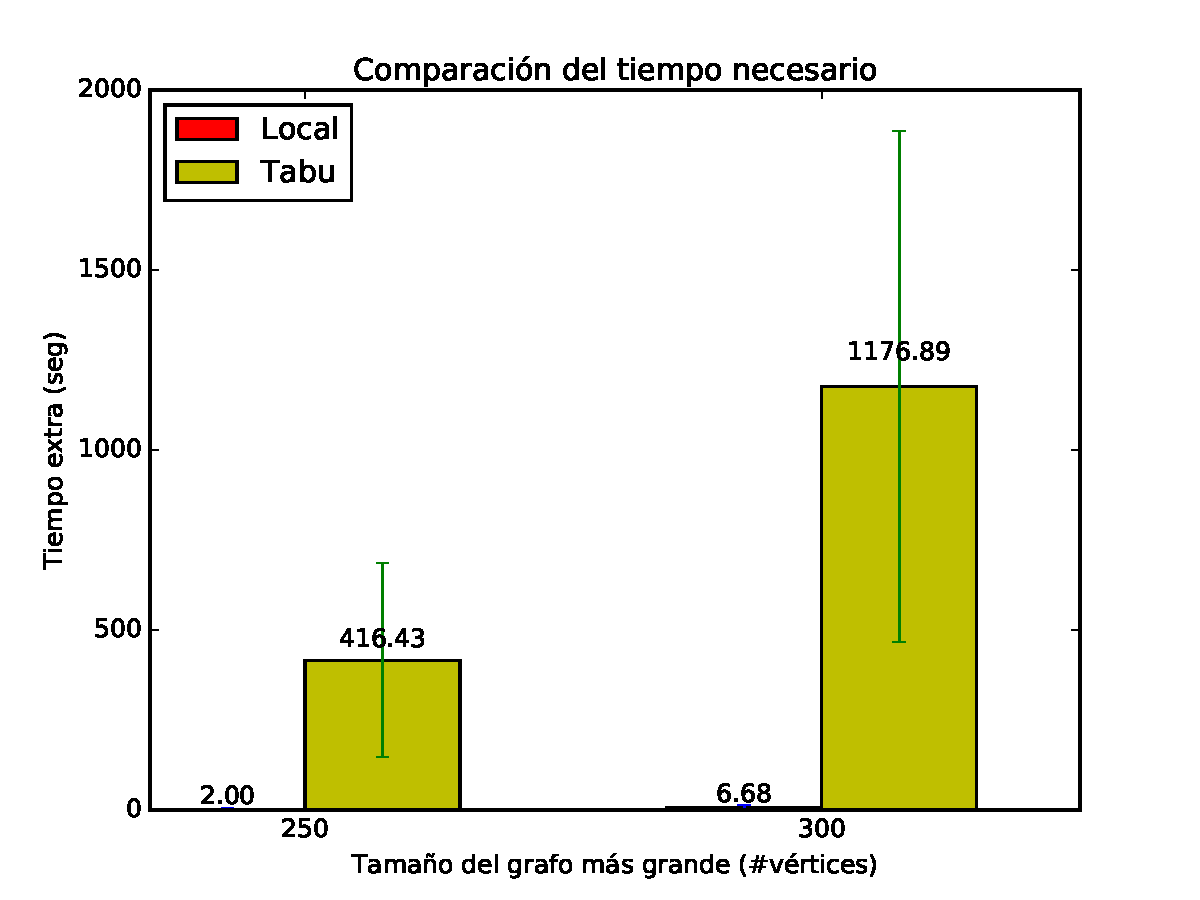
\includegraphics[width=1\textwidth]{graficos/problema_7/tiempo4.pdf}
  \caption{}
  \label{fig:7-tiempo3}
\end{minipage}%
\end{figure}

\begin{figure}[H]
\centering
\begin{minipage}{0.49\textwidth}
  \centering
    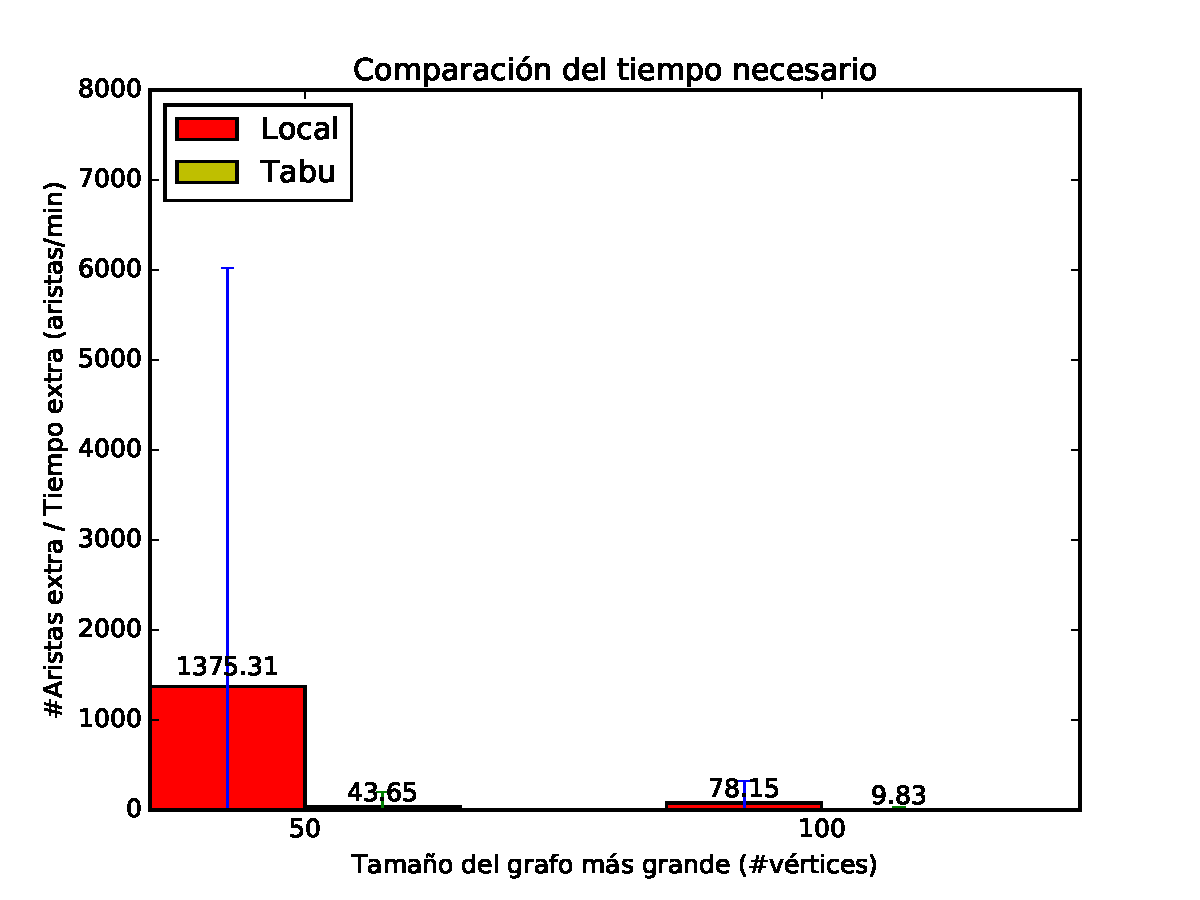
\includegraphics[width=1\textwidth]{graficos/problema_7/cociente0.pdf}
  \caption{}
  \label{fig:7-cociente1}
\end{minipage}%
\hspace{0.01\textwidth}
\begin{minipage}{0.49\textwidth}   
  \centering
    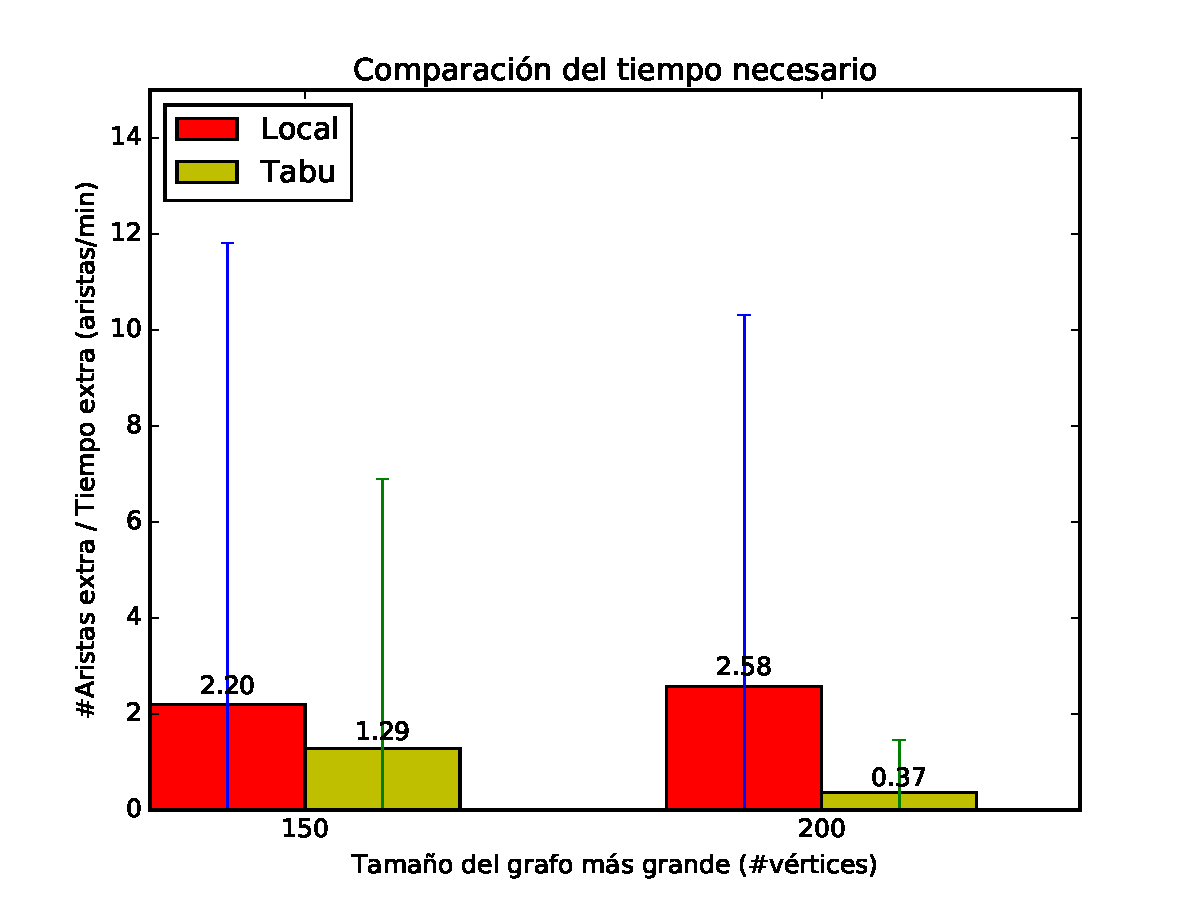
\includegraphics[width=1\textwidth]{graficos/problema_7/cociente2.pdf} 
  \caption{}
  \label{fig:7-cociente2}
\end{minipage}

\begin{minipage}{0.49\textwidth}
  \centering
    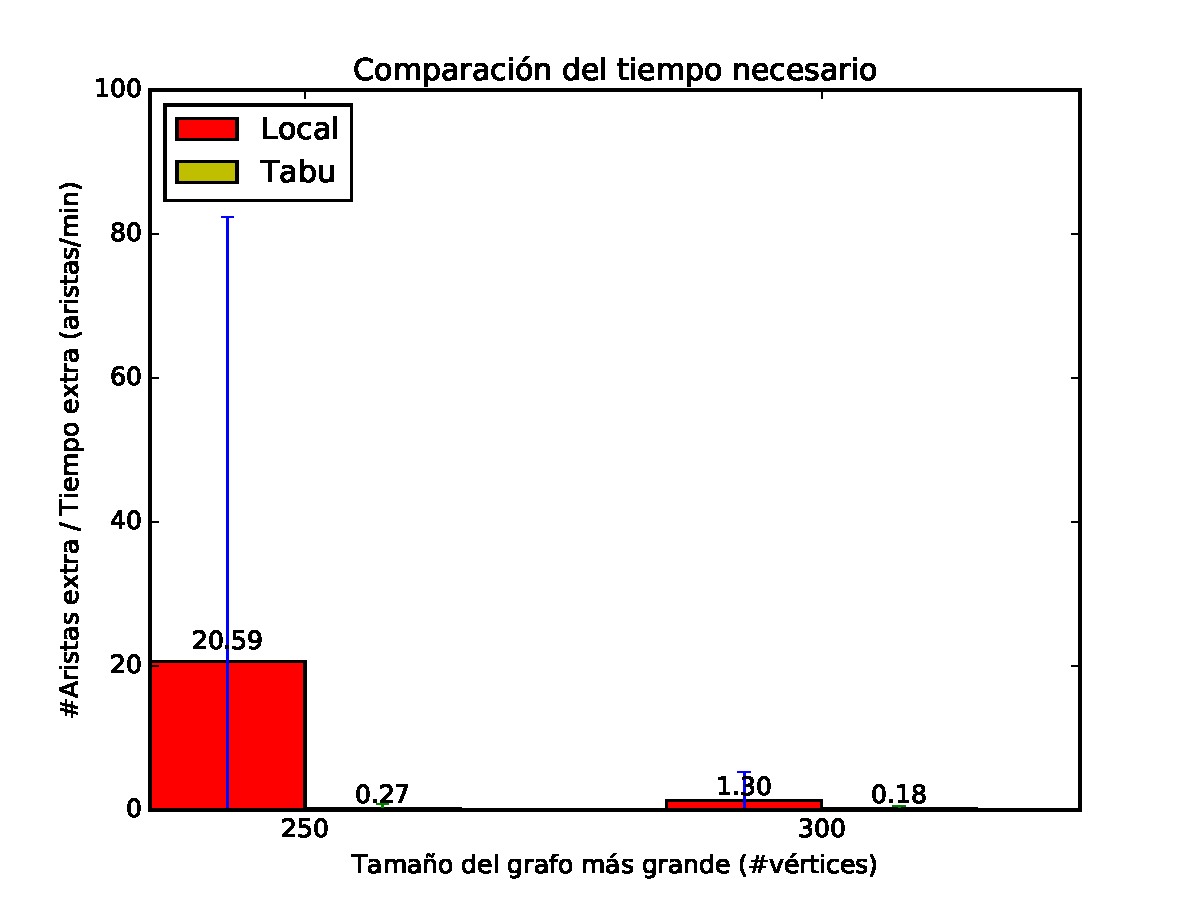
\includegraphics[width=1\textwidth]{graficos/problema_7/cociente4.pdf}
  \caption{}
  \label{fig:7-cociente3}
\end{minipage}%
\end{figure}

\subsection{Comparación con el algoritmo exacto}

Algo interesante que podemos preguntarnos es cómo se comparan nuestros algoritmos con el algoritmo exacto.

Sin embargo, como vimos anteriormente, el algoritmo exacto es extremadamente lento, por lo que un experimento ``clásico'', en el que se generan casos al azar y se corren los algoritmos sobre ellos no es viable.

Por esta razón, decidimos elegir una familia de grafos para la cual conozcamos de antemano, por sus características, la solución exacta, sin necesidad de correr el algoritmo exacto. 

Esta familia es precisamente la familia que encontramos como ``contraejemplo'' en el ejercicio del algoritmo goloso. Era la familia que nos permitía demostrar que el algoritmo no es $\alpha$-aproximado para ningún $\alpha > 0$. 

Recordemos los grafos y analicemos sus propiedades.


\begin{tikzpicture}[shorten >=1pt,auto,node distance=1.9cm,
                    semithick]
  \tikzstyle{every state}=[fill=red,draw=none,text=white]

	\node[state]	(0)		 		  {$2$};
	\node[state]	(1) [right of=0]  {$4$};
	\node[state]	(2) [below of=0]  {$3$};
	\node[state]	(3) [left of=0] 	  {$0$};
	\node[state]	(4) [above of=0]	  {$1$};
	\node[state]	(5) [right of=1]	  {$5$};
	\node[state]	(6) [above of=5]  {$6$};
	\node[state]	(7) [right of=6]  {$7$};
	\node[state]	(8) [right of=5]  {$8$};
	\node[state, fill=blue]	(9) [right of=8]	  {$0$};
	\node[state, fill=blue]	(10) [above of=9]  {$1$};
	\node[state, fill=blue]	(11) [right of=9]  {$2$};
	\node[state, fill=blue]	(12) [right of=10]  {$3$};


	\path	
		(0) edge[]				node {} (1)
         	edge[]				node {} (2)
         	edge[]				node {} (4)
         	edge[]				node {} (3)
		(1) edge[]				node {} (5)
		(5) edge[]				node {} (6)
		    edge[]				node {} (7)
		    edge[]				node {} (8)
		(6) edge[]				node {} (7)
		    edge[]				node {} (8)
		(7) edge[]				node {} (8)
		(9) edge[]				node {} (10)
		    edge[]				node {} (11)
		    edge[]				node {} (12)
		(10) edge[]				node {} (11)
		    edge[]				node {} (12)
		(11) edge[]				node {} (12);

\end{tikzpicture}

En nuestro caso utilizaremos una pequeña variación de este grafo (la única diferencia es que la arista que une a la estrella con el completo no sale de un brazo, si no de el centro de la estrella).

Como vimos anteriormente, el algoritmo goloso devuelve una solución muy mala siempre, dado que mapea al grafo completo azul con el grafo estrella rojo. 

Otra cosa que puede observarse es que, por como son nuestras heurísticas de búsqueda local, esa solución (la del goloso) es un mínimo local para todas estas soluciones. Esto puede chequearse muy fácilmente viendo la forma de los grafos y las soluciones (cualquier vecino a la solución del goloso es igual o peor que la solución del goloso).

Sin embargo, el tabú search viene a solucionar este problema, debido a la función de aspiración, que nos permite saltar a una solución aunque sea peor que la que tenemos, si todas lo son.

Enunciadas nuestras hipótesis sobre la experimentación, veamos los resultados.

\begin{figure}[H]
 \centering
	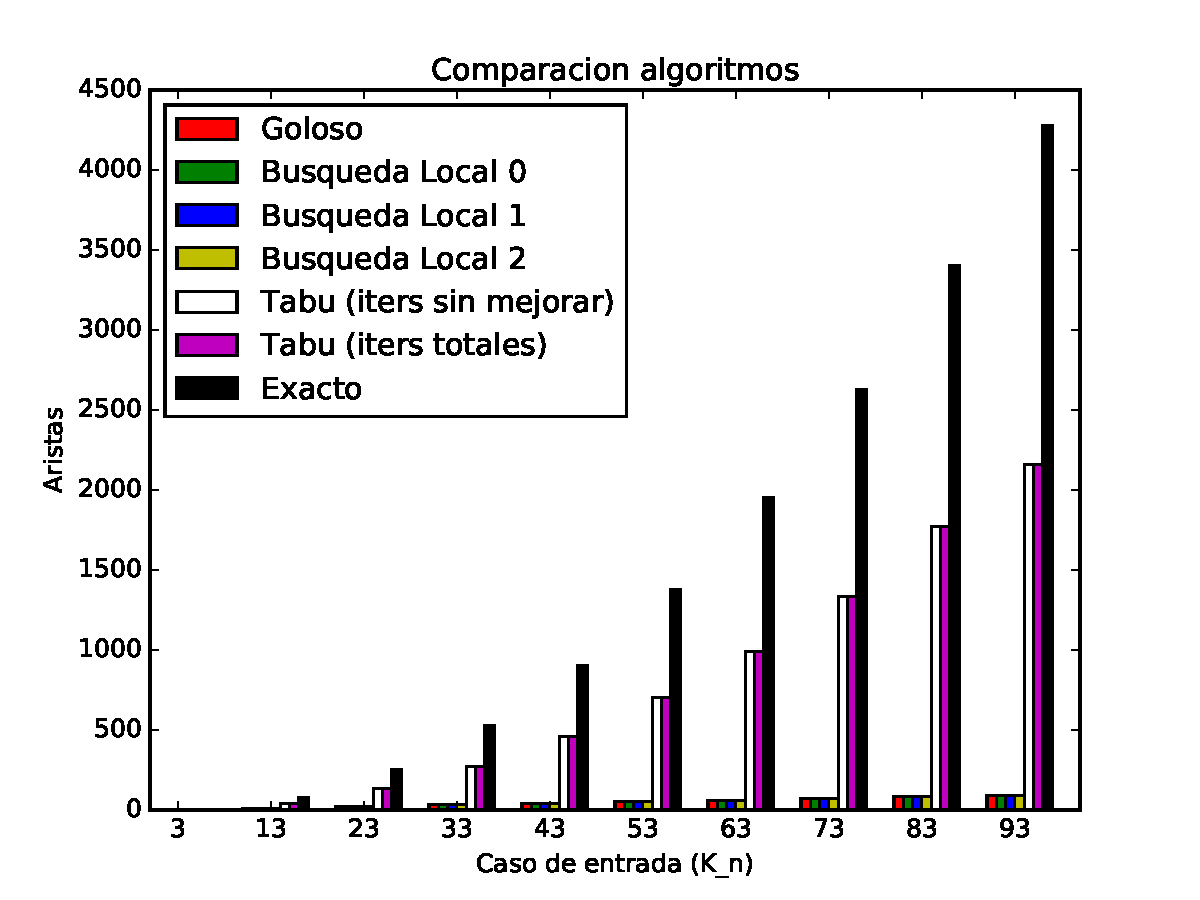
\includegraphics[width=0.9\textwidth]{graficos/problema_7/exacto0.pdf}
	\caption{}
	\label{fig:problema7-exacto0}
\end{figure}


Puede verse que sucede lo que esperábamos. Es decir, la solución del algoritmo goloso es muy mala, y la de las búsquedas locales no lo mejora.

Sin embargo, el tabú search permite mejorar mucho las soluciones. De todos modos, al igual que antes, no se observan diferencias notorias entre los dos criterios de parada del algoritmo: el secreto del éxito reside en las buenas vecindades que elegimos.

\subsection{Conclusiones}
Como cierre para las últimas tres secciones donde experimentamos y discutimos ampliamente sobre distintas heurísticas y metaheurísticas, pasamos en limpio algunas conclusiones.

Encontramos que la solución golosa para casos generales no resulta tan mala como se esperaba inicialmente. Incluso analizamos otra variante golosa mucho más rudimentaria en la que simplemente se mapeaban los nodos de mayor grado de cada grafo, y sorpresivamente no tuvo tan malos resultados. Sin embargo, como el otro era consistentemente mejor en calidad lo preferimos por sobre el más simple, aunque también fuese significativamente más rápido. 

Entre las búsqueda locales vimos que en muchos casos permitían mejorar la solución golosa, aunque en general nunca demasiado. Para obtener soluciones que sacarán levemente mayor diferencia teníamos que recurrir a una vecindad, que aunque se podía recorrer polinomialmente, en la práctica el costo a pagar era muy alto. 

Como propuesta superadora probamos distintas implementaciones de la metaheurística de búsqueda local \emph{tabu search} variando sus parámetros más clásicos. Lo que obtuvimos fue un resultado muy satisfactorio desde el punto de vista de la calidad, aunque nuevamente pagando un fuerte precio en tiempo. También vimos en esta sección que sigue estando lejos de ser un algoritmo exacto.

En definitiva, a la hora de escoger una u otra alternativa habrá que considerar fuertemente el contexto de uso: en un ámbito científico como el planteado por el problema posiblemente sea preferible recurrir a la búsqueda tabú aunque pueda requerir horas o días para obtener el resultado deseado, pues seguramente la situación resulte lo suficientemente delicada como para requerir la mejor solución posible. También es la mejor alternativa en general para instancias relativamente chicas. En contextos menos críticos donde se prefiera la velocidad, INTERCAMBIAR, REMPLAZAR o incluso la misma heurística golosa resultan alternativas más sensatas.  



\newpage

\section{Apéndice}

\subsection{Generación de grafos conexos aleatorios}
\label{subsec:grafos-aleatorios}

\begin{algorithm}[H]
  \begin{algorithmic}[1]
  \caption{Pseudocódigo del procedimiento para generar grafos conexos al azar}
  \label{algo:ap-1}
    \Procedure{grafo\_random}{\texttt{int} $n$, \texttt{int} $m$}$\rightarrow$ \texttt{Grafo}

    	\State $k_n \gets \{(0,1), (0,2), ..., (0,n), (1,2), (1,3), ..., (n-2, n-1)\}$
      \State $vertices \gets \{random.range(0, n)\}$ \Comment Empiezo con un vértice al azar
      \State $agm \gets \{\}$
      \While{$vertices$.size() $< n$}
         \State $aristas \gets$ ``aristas $(u,v)$ de $k_n$ tal que $u \in vertices$ y $v \not\in vertices$ o viceversa''
         \State $arista\_nueva \gets$ random.choice($aristas$)
         \State $agm.add(arista\_nueva)$
         \State $k_n.remove(arista\_nueva)$
         \State $vertices.add($``extremo de $arista\_nueva$ que no estaba en vertices''$)$
      \EndWhile
      \State \Comment Cuando termina este ciclo tenemos un árbol de $n$ vertices y $n-1$ aristas
      \State $grafo \gets agm$
      \While{$grafo$.size() $< m$}
         \State $arista \gets random.choice(k_n)$
         \State $grafo.add(arista)$
         \State $k_n.remove(arista)$
      \EndWhile
      \For{$arista \in grafo$}
         \State{$peso(arista) \gets random.random()$}
      \EndFor
      \Return $grafo$
		\EndProcedure
	\end{algorithmic}
\end{algorithm}


El algoritmo, se basa en generar un grafo conexo minimal (es decir, un árbol) de $n$ vértices.
Para lograr esto, técnicamente lo que hacemos es empezar con $K_n$, es decir, el grafo completo de $n$ vértices, con todos sus aristas de igual peso, y le encontramos un árbol generador mínimo utilizando Prim. Todo esto es obviamente trivial en este caso, dado que todas las aristas tienen igual peso, así que básicamente lo que hacemos es elegir una arista al azar en cada paso.

Luego, una vez que tenemos el árbol terminado, lo completamos con aristas al azar, hasta llegar al objetivo de $m$ aristas. 

Finalmente, se eligen pesos al azar para cada arista.


\newpage
\subsection{Partes relevantes del código}
\lstset{language=C++, breaklines=true, basicstyle=\footnotesize}
\lstset{numbers=left, numberstyle=\tiny, stepnumber=1, numbersep=5pt, tabsize=2}



\newpage
\printbibliography

\end{document}
